% !TeX root = ../main.tex

\chapter{玻色超流体中赝时间反演对称性保护的拓扑Bogoliubov激发模}

\section{研究背景}
在绪论中\ref{sec:tbt}节中我们已经详细讨论了传统(自由费米子)拓扑能带理论。特别地,我们已经知道针对拓扑绝缘体和拓扑超导体的三种内禀对称性(时间反演对称性、粒子-空穴对称性和手性对称性),有所谓的十重分类,见\ref{tenfoldway}小节。这里我们关注光晶格中弱相互作用超冷玻色子集体激发对应能带的拓扑。事实上我们已经知道这些激发谱的能带存在拓扑结构 \cite{Furukawa2015,Xu2016,Liberto2016}。
但是所有之前的工作都是关注的时间反演对称性被破坏的系统,
这些体系在二维有非零的陈数,
并且其与边界的手性模个数有一一关系,
这就是所谓的体边对应关系(见\ref{subsec:tebbc}小节)。
根据十重分类定义,这种激发谱的能带拓扑对应于A类的陈绝缘体。

归功于Kane和Mele,我们现在知道在二维存在一种被奇的时间反演对称性保护的拓扑态,即属于AII类的拓扑绝缘体。这种拓扑态有一对螺旋形的边界态,在同一边界沿着相反的方向传播;其存在与否是被一个体态的$\mathbb Z_2$拓扑数描述的。这个$\mathbb Z_2$拓扑数有很多等价的定义:比如用Pfaffian \cite{Kane2005}、时间反演极化 \cite{Fu2006} 和Wannier中心的流动 \cite{Yu2011} 来定义。注意最后一种定义是实践中最好用的,因为它不涉及需要固定规范的问题(见式\eqref{gaugeconstraint1})。
一个自然的问题是,类似的拓扑结构是否在玻色超流体的低能激发谱能带中存在呢?
如果是,
怎么定义对应的体拓扑数?
体边对应关系是否仍然成立?

以下我们展示AII类的拓扑结构确实在光晶格中玻色爱因斯坦凝聚体的Bogoliubov激发谱能带中存在,并且它是被一个赝时间反演对称性保护的,
后者是赝反幺正的,
并且其平方等于$-1$。
我们证明对应的体拓扑数也是一个$\mathbb Z_2$数,
并且之前提到的费米子情况的三个定义都可以在这里找到对应。

\section{Krein空间理论}\label{ksf}

在这一节我们简单介绍下Krein空间理论,并且把第\ref{ch2}章里讨论的玻色型BdG方程的求解用Krein空间理论重新描述。 \cite{Peano2018,Bender2019,Lein2019}。

一个Krein空间$(\mathcal K,J)$就是一个带有基本对称性$J$的Hilbert空间$\mathcal K$,这里$J$是一个线形算符,并且满足$J^2=1$和$J=J^\dagger$。等价地,算符$J$是一个基本对称当且仅当
\begin{equation}
	J^2=1, \qand \expval{J\phi,J\psi}=\expval{\phi,\psi},\ \forall \phi,\psi\in \mathcal K,\nonumber
\end{equation}
这里$\expval{\cdot,\cdot}$是通常意义上的定义在Hilbert空间$\mathcal K$的内积。我们说一个Krein空间是实的,如果它有一个实的结构,并且存在一个实的幺正算符$Q$满足其平方为$\pm 1$,还和$J$(反)对易 \cite{SchulzBaldes2016}。

我们定义一个赝内积,
\begin{equation}
	\krin{\phi,\psi} := \expval{\phi,J \psi}. \label{defkip}
\end{equation}
注意到所有建立在通常内积上的概念都有关于赝内积的定义。首先,赝伴随矩阵被定义为$A^\sharp=J A^\dagger J$,
它满足$\krin{A^\sharp \phi,\psi}=\krin{\phi,A\psi}$。
然后赝厄米矩阵指$A^\sharp=A$,
即它是关于赝内积厄米的;
赝幺正指$A^\sharp=A\inv$,
即它的赝伴随矩阵就是它的逆矩阵;
赝反幺正是关于赝内积反线形的,
即$\krin{A\phi,A\psi}=\krin{\phi,\psi}^*=\krin{\psi,\phi}$。
最后,赝正交投影算子$\Pi$是赝厄米的,
并且它的平方等于它自己,
$\Pi^2=\Pi=\Pi^\sharp$,
这暗示了$\Pi$和$\Pi^\dagger$是通过一个相似变换联系的。

和厄米性不同,赝厄米性并不总是暗示实谱。但是所谓的Krein-spectral算符,它被定义为满足
\begin{equation}
	\tilde H=UHU\inv =UHU^\sharp=\tilde H^\sharp =\tilde H^\dagger,\nonumber
\end{equation}
其显然是有实普。特别地,那些关于赝内积非负的算符自动是Krein-spectral算符\cite{Peano2018,Colpa1978}.

对于一个玻色型BdG系统,我们有实的$(1,-1)$类Krein空间 \cite{SchulzBaldes2016},这里$J=\Sigma_3$,
$Q=\Sigma_1$。
有效哈密顿量式\eqref{hkbdg}是带有实对称的赝厄米矩阵。
Bogoliubov变换矩阵$T_{\boldsymbol k}$式\eqref{deftk}是一个带有实对称的赝幺正矩阵.

式\eqref{tkpu}可以被重写为一个赝内积的形式,
\begin{equation}\label{orthogonal conditions}
	\begin{split}
		\krin{u^\pm_n(\boldsymbol k),u^\pm_m(\boldsymbol k)} &=\pm \delta_{mn},\\
		\krin{u^\pm_n(\boldsymbol k),u^\mp_m(\boldsymbol k)} &=0.
	\end{split}
\end{equation}
其中$\ket{u^\pm_n(\boldsymbol k)}$是$H^\eff_{\boldsymbol k}$的右本征向量,
其对应的本征值为$\pm E_n(\pm \boldsymbol k)$。
这里的赝正交投影算子$\Pi$是赝厄米的,并且一般是非厄米的,它的形式是
\begin{equation}\label{projop}
	\Pi_{n,\boldsymbol k}=\pm \ketbra{u^\pm_n(\boldsymbol k)}{u^\pm_n(\boldsymbol k)}\Sigma_3.
\end{equation}
从这开始,除非单独声明,我们将只关注粒子空间,因为由于粒子-空穴对称性,空穴激发只是前者的复制。为了避免杂乱,我们也省略表示粒子空间的上指标``+".

最后我们简单解释下如何在拓扑能带理论中处理Nambu-Goldstone(NG)模。
NG模是一种由于系统连续对称性破缺导致的无能隙模,
它们一般不满足式\eqref{orthogonal conditions}给出的关系\cite{Takahashi2015,Watanabe2020}。
但是我们总可以通过加一个无穷小外场显式地破坏对应的对称性来去除这些NG模。
例如零能的声模总可以通过给化学势从负方向加一个无穷小的值$\mu\rightarrow \mu-0^+$,
来打开一个无穷小的能隙。
在以下讨论中,为了简便,我们总假设NG模有一个无穷小的能隙。
事实上,
正如我们在下一节末尾会提到的那样,
当我们考虑体边对应关系来推断螺旋型、能隙中间的边界态时,
我们总可以完全避免去讨论最底部的粒子能带的拓扑,
所以这些NG模拓扑的具体定义也是不相关\cite{Furukawa2015}。

\section{赝时间反演对称性导致的$\mathbb Z_2$不变量}\label{sec2}

\subsection{赝时间反演对称性}

对于一个玻色系统,
一般的时间反演对称算符的平方是等于$+1$的 \cite{Sakurai2014}。
我们定义一个赝时间反演算符$\mathcal{T}=PK$,
它的平方等于$-1$。
这里$P$是一个$\boldsymbol k$无关的赝幺正矩阵。
根据定义我们有$\mathcal T$是一个赝反幺正矩阵\footnote{
这个证明和通常的奇的时间反演对称性类似。考虑
\begin{eqnarray*}
	\krin{\phi,\mathcal{T}\psi} &=& \phi^*_i (\Sigma_3P)_{ij} \psi^*_j\\
	&=& \psi_j^* (P^T\Sigma_3)_{ji}\phi^*_i\\
	&=& \krin{\psi,\Sigma_3 P^T\Sigma_3 K\phi},
\end{eqnarray*}
然后将$\phi$换成$\mathcal{T}\phi$,
并且利用$P$的赝幺正性,
\begin{eqnarray*}
	\krin{\mathcal{T}\phi,\mathcal{T}\psi} &=& \krin{\psi,\Sigma_3 P^T \Sigma_3 KPK\phi}\\
	& = &\krin{\psi,\phi}.
\end{eqnarray*}
所以$\mathcal T$确实是赝反幺正的。}。

我们说一个玻色型BdG系统是满足赝时间反演对称性的,如果
\begin{equation}
	\mathcal{T} H^\eff_{\boldsymbol k} \mathcal{T}\inv=H_{-\boldsymbol k}^\eff.\label{PTRS}
\end{equation}
类似对于费米子的奇的时间反演对称性,
这个对于玻色子的赝时间反演对称性也暗示了玻色型Kramers对的存在:
对于每个$H^\eff_{\boldsymbol k}$的右本征向量$\ket{u_n(\boldsymbol k)}$,
由于式\eqref{PTRS},
$\mathcal{T}\ket{u_n(-\boldsymbol k)}$也是一个右本征向量,
其对应的本征值是$E(-\boldsymbol k)$。
在赝时间反演对称的动量$\boldsymbol{\Lambda}$,
这两个右本征态有相同的本征能量;
并且他们是关于赝内积正交的\cite{Kondo2019}。
这个正交性可以通过考察等式$\krin{\mathcal{T}\phi,\mathcal{T}\psi}=\krin{\psi,\phi}$,
通过令$\ket{\psi}=\ket{u_n(\boldsymbol{\Lambda})}$和$\ket{\phi}=\mathcal{T} \ket{\psi}$,
由于$\mathcal{T}^{2}=-1$,
等式两边必须分别等于零,
从而导出玻色型Kramers对,$\ket{u_n(\boldsymbol{\Lambda})}$和$\mathcal{T} \ket{u_n(\boldsymbol{\Lambda})}$ 的正交性。

\subsection{Pfaffian方法}

类比于Kane和Mele构造$\mathbb Z_2$不变量的方法\cite{Kane2005},
我们考虑赝时间反演算符在赝内积下,
关于两个$H^\eff_{\vb k}$的右本征向量的交叠矩阵$\krin{u_n(\vb k),\mathcal T u_m(\vb k)}$。
注意由于$\mathcal T$是赝反幺正的,
这个交叠矩阵显然是反对称并且平方等于$-1$。
假设没有其他简并,
那么这个交叠矩阵是$2\times 2$的,
\begin{equation}\label{overlap}
	\krin{u_n(\vb k),\mathcal T u_m(\vb k)}=\epsilon_{nm} P(\vb k),
\end{equation}
这里$P(\vb k)$是该矩阵的Pfaffian,
\begin{equation}
	P(\vb k)=\pf[\krin{u_n(\vb k),\mathcal T u_m(\vb k)}].\label{defpf}
\end{equation}
通过一个$\mathrm{U}(2)$变换,
$\ket{u_n(\vb k)} \rightarrow  R_{nm}(\vb k)\ket{u_m(\vb k)}$,
这个Pfaffian变成$P(\vb k) \rightarrow  \det[R^*(\vb k)]P(\vb k)$ [参考式\eqref{pdetrp}]。
所以$P(\vb k)$是在$\mathrm{SU}(2)$旋转下不变的,
但是不是$\mathrm{U}(1)$变换不变的。
因为后者会产生一个全局相位。
尽管如此,
$\abs{P(\vb k)}$仍是$\mathrm{U}(2)$规范不变的。
在赝时间反演不变的动量处$\boldsymbol{\Lambda} $,
由于玻色型Kramers对的存在,
非对角元有单位模,
即$\abs{P(\boldsymbol{\Lambda} )}=1$。
我们定义一个缝合矩阵$B(\vb k)$,用来联系赝时间反演关联的一对本征态,分别在$\vb k$和$-\vb k$,
\begin{equation}
	\ket{u_m(-\vb k)}=B^*_{mn}(\vb k)\mathcal T \ket{u_n(\vb k)},\label{sewingm}
\end{equation}
用它可以导出$P(-\vb k)=\det[B(\vb k)] P^*(\vb k)$,见式\eqref{pfatkmk}。
所以每当Pfaffian在一个动量处等于零时,
在相反动量处也等于零,并且它们有相反的“旋度”。
这导致Pfaffian的零点对在有赝时间反演对称性时是一个$\mathbb Z_2$不变量,和费米子时情况一样\cite{Kane2005}。
等价地,$P(\vb k)$在半个第一布里渊区相位的绕树\begin{equation}
	I= \frac{1}{2\pi i}\oint_C \dd{\vb k}\cdot\nabla_{\vb k}\log[P(\vb k)],\nonumber
\end{equation}
是一个有赝时间反演对称性玻色型BdG系统$\mathbb Z_2$不变量。
注意到,我们可以很简单地证明Pfaffian在粒子能带和在空穴能带有直接联系,见式\eqref{holepfaffian}],且有$I_\textnormal{particle}=I_\textnormal{hole}$。

\subsection{赝时间反演极化}
类比于Fu和Kane\cite{Fu2006},我们同样可以定义一个赝时间反演极化来表征这个$\mathbb Z_2$不变量。这个方法也是Engelhardt和Brandes对于玻色型BdG系统构造的辛“电荷”极化的直接推广\cite{Engelhardt2015}。把$k_2$(看作时间$t$)固定在$k_2=0$或$\pi$(即$t=0$或$T/2$),
同时令$k_1=k$,于是我们得到一个有效的一维系统。
假设这里没有其他简并,
$N$个粒子能带可以被分成$N/2$个赝时间反演对。
第$\lambda $个($\lambda =1,2 \dots ,N/2$)对被记为$\ket{u_{\lambda }^{(l)}(\vb k)}$,
这里$l=1,2$标记一个赝时间反演对中的两个态。
由于赝时间反演对称性,
对每一对,$l=2$的在$\vb k$的本征态的赝时间反演伙伴和$l=1$在$-\vb k$的本征态最多差一个相位因子\cite{Fu2006},
\begin{subequations}\label{12x}
\begin{eqnarray}
	\ket{u_{\lambda }^{(1)}(-k)} &=& -\eu^{\iu\chi_{k,\lambda }}\mathcal T \ket{u_{\lambda }^{(2)}(k)},\\
	\ket{u_{\lambda }^{(2)}(-k)} &=& \eu^{\iu\chi_{-k,\lambda }}\mathcal T \ket{u_{\lambda }^{(1)}(k)}.
\end{eqnarray}
\end{subequations}
这里第二个方程可由第一个方程导出。
我们定义对于第$\lambda$对的部分极化
\begin{equation}
	P_{\lambda }^{(l)}=\frac{1}{2\pi}\int_{-\pi}^\pi\dd{k} A_{\lambda }^{(l)}(k),\nonumber
\end{equation}
其中Berry联络是 \cite{Shindou2013}
\begin{equation}\label{berryconnectionpartial}
	A^{(l)}_{\lambda }(k) = i \krin{u_{\lambda }^{(l)}(k),\partial_k u_{\lambda }^{(l)}(k)}.
\end{equation}
注意到两个部分极化的和是辛推广的“电荷”极化\cite{Engelhardt2015}。
这里我们考虑它们的差,
\begin{equation}
	\tilde P_{\lambda }=P^{(1)}_\lambda -P^{(2)}_\lambda,\nonumber
\end{equation}
作为Fu和Kane提出的时间反演极化的辛推广 \cite{Fu2006},它满足(证明见\ref{trp1})
\begin{equation}
	(-1)^{\tilde P_\lambda }=\frac{\sqrt{\det[B_\lambda (0)]}}{\pf[B_\lambda (0)]}\frac{\sqrt{\det[B_\lambda (\pi)]}}{\pf[B_\lambda (\pi)]},\label{trp}
\end{equation}
其中$B_\lambda (k)=B(k,0)$或$B(k,\pi)$是对于第$\lambda $对的,定义在式\eqref{sewingm}的缝合矩阵。
这里的符号歧义是通过要求$\sqrt{B_\lambda (k)}$是在$k\in [0,\pi]$连续。
根据文献\cite{Fu2006}的讨论,
赝时间反演极化在半个循环的变化,物理上追踪了一对Wannier态位置之差,可以定义一个$\mathbb Z_2$不变量(
即,这些Wannier态是否交换了对象),
\begin{equation}
	\Delta_\lambda =\tilde P_\lambda (T/2)-\tilde P_\lambda (0)\mod 2.\label{z2PTRp}
\end{equation}
利用式\eqref{trp},
我们可以等价地把式\eqref{z2PTRp}写成
\begin{equation}\label{z2dl}
	(-1)^{\Delta_\lambda }=\prod_{i=1}^4\frac{\sqrt{\det[B_\lambda (\Gamma_i)]}}{\pf[B_\lambda (\Gamma_i)]}.
\end{equation}
容易看出,$\Delta_\lambda $对于粒子能带和他的对应的空穴能带是一样的,
即$\Delta_\lambda ^{\textnormal{particle}}=\Delta_\lambda ^{\textnormal{hole}}$,
参考式\eqref{bhole}.

通过强加所谓的赝时间反演限制\cite{Fu2006},
\begin{equation*}
	\begin{split}
		\ket{u^{(1)}_\lambda (-k,-t)} &=\mathcal T\ket{u^{(2)}_\lambda (k,t)},\\
		\ket{u^{(2)}_\lambda (-k,-t)} &=-\mathcal T\ket{u^{(1)}_\lambda (k,t)},
	\end{split}
\end{equation*}
这个$\mathbb Z_2$不变量也可以被看成是一种阻塞(obstruction)。
在这个观点下,我们可以得到利用阿贝尔Berry联络
\begin{equation}\label{berryconnection}
	\vb A_\lambda (\vb k)= \sum_{l=1,2} i\krin{u_\lambda ^{(l)}(\vb k),\nabla_{\vb k} u_\lambda ^{(l)}(\vb k)},
\end{equation}
和阿贝尔Berry曲率
\begin{equation}
	F_{\lambda }(\vb k) =\sum_{l=1,2} [\nabla_{\vb k}\times \vb A_{\lambda }^{(l)}(\vb k)]_z,\nonumber
\end{equation}
定义的一个$\mathbb Z_2$不变量表达式 \cite{Kondo2019}
\begin{equation}\label{fukui}
	\begin{split}
		&\quad \tilde \Delta_\lambda =\\
	& \frac{1}{2\pi}\Bqty{\oint_{\partial \textnormal{HBZ}}\dd{\vb k}\cdot\vb A_\lambda (\vb k)-\int_{\textnormal{HBZ}}\dd[2]{k}F_\lambda (\vb k)}\mod 2,
	\end{split}
\end{equation}
这里$\textnormal{HBZ}$和$\partial\textnormal{HBZ}$指一半的第一布里渊区和它的边界,注意这里的一半是指里面没有任意两个点是由赝时间反演对称性联系的。
类似文献\cite{Fu2006}的附录部分,可以证明$\tilde \Delta_\lambda =\Delta_\lambda $,
以及它们与Pfaffian方案是等价的。

\subsection{通过Wannier中心流动定义$\mathbb Z_2$不变量}
上面提到的所有定义$\mathbb Z_2$不变量的方法都有需要固定规范。这里我们推广Yu等人提出的一种非常实用的计算方法\cite{Yu2011},
它没有固定规范的问题,因而在做数值计算时是非常有用的。

仍然考虑有效的一维系统(把$k_2$固定),
我们按照通常情况一样定义位置算符$\hat X=\sum_{i\alpha}e^{i \boldsymbol{\delta}_1\cdot\vb r_i}\ketbra{i\alpha}{i\alpha}$ \cite{Resta2000},
这里$\ket{i\alpha}=\ket{i}\otimes\ket{\alpha}=a^\dagger_{\vb r_i \alpha}\ket{0}$,$\boldsymbol{\delta}_1=\vb b_1/N_1$,$\vb b_1$是倒格子单位向量,$N_1$是有效一维系统的晶胞数。

所谓的Wannier态就是被限制在“占据态”子空间的位置算符的本征态\cite{Kivelson1982},
$\hat X_P=\hat P\hat X \hat P$。
这里对于“占据态”空间的投影算符是(参考式\eqref{projop}),
\begin{equation}
	\hat P = \sum_{n\leq n_\tmax,k_1} \ketbra{\psi_n(\vb k)}{\psi_n(\vb k)}\Sigma_3,\nonumber
\end{equation}
其中$\ket{\psi_n(\vb k)}=\ket{\vb k}\otimes\ket{u_n(\vb k)}$是Bloch本征态,
$\ket{\vb k}=M^{-1/2} \sum_i e^{-i\vb k\cdot\vb r_i}\ket{i} $。
利用
\begin{equation*}
	\krin{\psi_{n}(\vb k),\hat X \psi_{n'}(\vb k')} = \delta_{\vb k+\boldsymbol{\delta}_1,\vb k'}\krin{u_{n}(\vb k),u_{n'}(\vb k+\boldsymbol{\delta}_1)},
\end{equation*}
被投影的位置算符可写作
\begin{equation*}
\begin{split}
	\hat X_P=\sum_{n,n'\leq n_\tmax}\sum_{k_1}\bigg[\krin{u_{n}(\vb k),u_{n'}(\vb k+\boldsymbol{\delta}_1)}\\
	\times \ketbra{\psi_{n}(\vb k)}{\psi_{n'}(\vb k+\boldsymbol{\delta}_1)}\Sigma_3\bigg]
\end{split}
\end{equation*}
我们考虑$\hat X_P$的$N_1$次方,
\begin{equation*}
	\hat X_P^{N_1}=\sum_{m,n\leq n_\tmax}\sum_{k_1}\bqty{W_{\vb k}}_{mn}\ketbra{\psi_m(\vb k)}{\psi_n(\vb k)}\Sigma_3
\end{equation*}
这里所谓的Wilson环算符$W_{\vb k}$被定义为
\begin{equation}
	W_{\vb k} =M^{(\vb k,\vb k+\boldsymbol{\delta}_1)} M^{(\vb k+\boldsymbol{\delta}_1,\vb k+2\boldsymbol{\delta}_1)}  \dots  M^{(\vb k+(N_1-1)\boldsymbol{\delta}_1,\vb k)},\label{wilsonloop}
\end{equation}
其中$\bqty{M^{(\vb k,\vb k+\boldsymbol{\delta}_1)}}_{mn} =\krin{u_{m}(\vb k),u_n(\vb k+\boldsymbol{\delta}_1)}$。
在$\abs{\boldsymbol{\delta}}_1\rightarrow 0$极限下,
我们有$\bqty{M^{(\vb k,\vb k+\boldsymbol{\delta}_1)}}_{mn}\rightarrow e^{-i[\mathcal A_1(\vb k)]_{mn} dk_1}$,
其中的非阿贝尔规范场$\mathrm{U}(n_m)$被定义为
\begin{equation}\label{nonaa}
	[\mathcal A_{1}(\vb k)]_{mn}=i \krin{u_m(\vb k),\partial_{k_1} u_n(\vb k)},
\end{equation}
然后式\eqref{wilsonloop}变成$\mathrm{U}(n_m)$Wilson环,
$W_{\vb k}=P\exp\bqty{\int_{-\pi}^\pi -i\mathcal A_1(\vb k)dk_1}$ \cite{peskin1995an}。

$W_{\vb k}$的本征值是与$k_1$无关的。在$\ket{u_n(\vb k)}$的$\mathrm{U}(n_m)$规范变换下,它也是不变的,证明见\ref{wlp}。
这些本征值被用$w_n=\abs{w_n}e^{i\theta_n}$表示,
这里$n=1, \dots ,n_\tmax$,
并且$\theta_n\in (-\pi,\pi]$。
所以$\hat X_P$的本征值,
作为$w_n$的第$N_1$次方根,
是$w_{n,j}=\exp[i\theta_n/N_1+i 2\pi j/N_1 +(\log\abs{w_n})/N_1]$,
其中$j=1, \dots ,N_1$。
最后,
Wannier中心就是$w_{n,j}$的相位,
\begin{equation}
	\expval{x}_{n,j}=\frac{N_1}{2\pi}\arg w_{n,j}=\expval{x}_n+j,\quad \expval{x}_n=\theta_n/2\pi\nonumber
\end{equation}
根据这个定义,它是可以有任意晶格单位向量平移的。

由于赝时间反演对称性,Wilson环算符的本征值在$k_2$和$-k_2$处是一样的;
而且在赝时间反演不变的动量处,
本征值至少是双重简并的(证明见\ref{wlp})。
所以,从$k_2=-\pi$出发,
每一对Wannier中心会先分开,
然后在$k_2=0$处又汇合。
对于$k_2>0$,
这个行为和前诉行为是关于$k_2=0$面镜像对称的。
根据费米子情况下一样的原因\cite{Yu2011},
所有$n_\tmax/2$对Wannier中心的绕数和是一个$\mathbb Z_2$不变量。
这个定义和之前所有定义的等价性,可类似于文献\cite{Yu2011}的附录那样得到。


\subsection{来自额外的空间反演对称性的简化}
最后我们指出如果有一个额外的空间反演对称性,
那么这个$\mathbb Z_2$不变量式\eqref{z2dl}有一个简化的表达式,
\begin{equation}\label{isz2}
	(-1)^{\Delta_\lambda }=\prod_i \xi_\lambda (\boldsymbol{\Lambda} _i),
\end{equation}
这里$\xi_\lambda (\boldsymbol{\Lambda} _i)$是第$\lambda $对能带里其中一个在赝时间反演不变动量$\boldsymbol{\Lambda} _i$处的空间反演对称算符的本征值。
类比于Fu和Kane在费米子情况里的讨论\cite{Fu2007},
我们通过构造一个全局连续的横向规范$\vb A_\lambda (\vb k)=0$,
在这个规范下证明式\eqref{isz2}。

我们说一个玻色型BdG系统有空间反演对称性,
如果存在一个空间反演算符$\mathcal P$,
满足
\begin{equation}
	\mathcal P H^\eff_{\vb k} \mathcal P\inv = H^\eff_{-\vb k}.\nonumber
\end{equation}
这里$\mathcal P$是$\vb k$无关的,赝幺正的,赝厄米的(参考式\eqref{prfcuni}和式\eqref{prfcansy}),
平方等于1,并且和赝时间反演算符$\mathcal T$对易。
根据定义,
我们有
\begin{equation}
	\mathcal P\mathcal T H^\eff_{\vb k} (\mathcal P\mathcal T)\inv = H^\eff_{\vb k},\nonumber
\end{equation}
即所有能带至少是双重简并的,在每一个$\vb k$。
可以直接证明,在赝时间反演不变的动量处,
每个Kramers对都有相同的空间反演算符本征值,
所以在式\eqref{isz2}中,我们不用担心对第$\lambda $对由赝时间反演算符关联的对里,应该选取哪个来计算。
另一个直接对事实是Berry曲率$F_\lambda (\vb k)$必须处处为零,
因为它同时是关于$\vb k$对奇和偶函数,
由于赝时间反演对称性和空间反演对称性。
现在我们在任意规范下定义一个幺正的、反对称的缝合矩阵$C$,
\begin{equation}
	\ket{u_m(\vb k)}= -C^*_{mn}(\vb k)\mathcal P\mathcal T\ket{u_n(\vb k)}.\label{sewmatcdef}
\end{equation}
假设没有其他简并,上述矩阵是$2\times 2$的,由$\lambda $标记的。
$C_\lambda (\vb k)$的Pfaffian有单位模长,并且它相位的梯度是与Berry联络式\eqref{berryconnection}联系的(见式\ref{gfusingc1}),
\begin{equation}\label{gfusingc}
	\begin{split}
		\vb A_\lambda (\vb k) &=-\frac{i}{2}\tr[C^\dagger_\lambda (\vb k) \nabla_{\vb k}C_\lambda (\vb k)]\\
		&=-i \nabla_{\vb k}\log \pf[C_\lambda (\vb k)].
	\end{split}
\end{equation}
通过选取一个合适的规范,我们可以令$\pf[C_\lambda (\vb k)]=1$,
然后Berry联络为零。
由于\ref{cbrelation1}
\begin{equation}\label{cbrelation}
	C_\lambda (-\vb k)=B_\lambda (\vb k)C^*_\lambda (\vb k) B^T_\lambda (\vb k),
\end{equation}
和$\pf[XAX^T]=\pf[A]\det[X]$,
这个规范也保证了$\det[B_\lambda (\vb k)]=1$。
最后,从式\eqref{smb},
我们有
\begin{equation}\label{bc1}
	[B(\boldsymbol{\Lambda} _i)]_{ll'}=\krin{\psi_\lambda ^{(l)}(\boldsymbol{\Lambda} _i),\mathcal P(\mathcal P\mathcal T)\psi_\lambda ^{(l')}(\boldsymbol{\Lambda} _i)}
\end{equation}
这里$\ket{\psi_\lambda ^{(l)}(\boldsymbol{\Lambda} _i)}=e^{i\boldsymbol{\Lambda} _i\cdot\vb r}\ket{u_\lambda ^{(l)}(\boldsymbol{\Lambda} _i)}$是Bloch本征态。
由于$[H,\mathcal P]=0$,
$\ket{\psi_\lambda(\boldsymbol{\Lambda} _i)}$也是$\mathcal P$的本征态,
其本征值是$\xi_\lambda =\pm 1$。
利用式\eqref{cdefanother},
式\eqref{bc1}导出$B_\lambda (\boldsymbol{\Lambda} _i)=\xi_\lambda (\boldsymbol{\Lambda} _i)C_\lambda (\boldsymbol{\Lambda} _i)$,
这在横向规范下给出$\pf[B_\lambda (\boldsymbol{\Lambda} _i)]=\xi_\lambda (\boldsymbol{\Lambda} _i)\pf[C_\lambda (\boldsymbol{\Lambda} _i)]=\xi_\lambda (\boldsymbol{\Lambda} _i)$。
总之,我们有$\sqrt{\det[B_\Lambda (\boldsymbol{\Lambda} _i)]}/\pf[B_\Lambda (\boldsymbol{\Lambda} _i)] =\xi_\Lambda (\boldsymbol{\Lambda} _i)$,
而式\eqref{isz2}则直接从式\eqref{z2dl}得到。

根据体-边对应,螺旋隙间的、在赝时间反演不变动量处的边界态的出现(消失)与$\mathbb Z_2$不变量等于一(零)存在一一对应关系。
注意到对于在第$n$和第$(n+1)$个粒子能带间的能隙,
对应的$\mathbb Z_2$不变量是通过算所有在第$n+1$个能带以下的能带,
这也包含了所有的空穴能带。
由于我们已经证明了一对粒子能带和它们对应的一对空穴能带有相同的$\mathbb Z_2$不变量,
所以我们可以等价地算所有第$n$个能带以上的能带的贡献。
这么做一个额外的好处是我们可以避免讨论在最低的粒子能带处出现的NG模\cite{Furukawa2015}。




\section{两个玩具模型}\label{sec3}
这一节我们通过具体计算两个可以在冷原子系统中实现的玩具模型:Kane-Mele模型和Bernevig-Hughes-Zhang模型,来考察激发谱的拓扑性质。
具体地,我们将用两种方案计算体拓扑数(即作为一个阻塞和作为Wannier中心流动),并且数值的确认体边对应关系。当系统有空间反演对称性时,我们同时也确认式\eqref{isz2}的正确性。

\subsection{Kane-Mele-Bose-Hubbard模型}
我们的第一个例子是Kane-Mele-Bose-Hubbard(KMBH)模型。
历史上,Kane-Mele模型\cite{Kane2005}是Haldane的六角晶格模型\cite{Haldane1988}的时间反演对称版本的推广。
注意到后者已经在冷原子体系中被Esslinger的实验组实现,我们预期这个模型也可以类似地实现。

自由哈密顿量部分如下
\begin{equation}\label{KMBHh0}
	H_0 = -t\sum_{\expval{i,j}}a^\dagger_i a_j-i\lambda _s\sum_{\krin{i,j}} v_{ij} a^\dagger_i s_3 a_j - \lambda_v \sum_i \xi_i a^\dagger_i a_i,
\end{equation}
其中$a^{(\dagger)}_i$是一个在格点$i$的玻色型湮灭(产生)算符,其赝自旋指标被忽略。
上式中第一项描述最近邻跃迁;第二项描述次紧邻带相位的跃迁,并且对于两种赝自选,有相反的相位,
见图\ref{KMBHlattice}。%
\begin{figure}
    \centering
	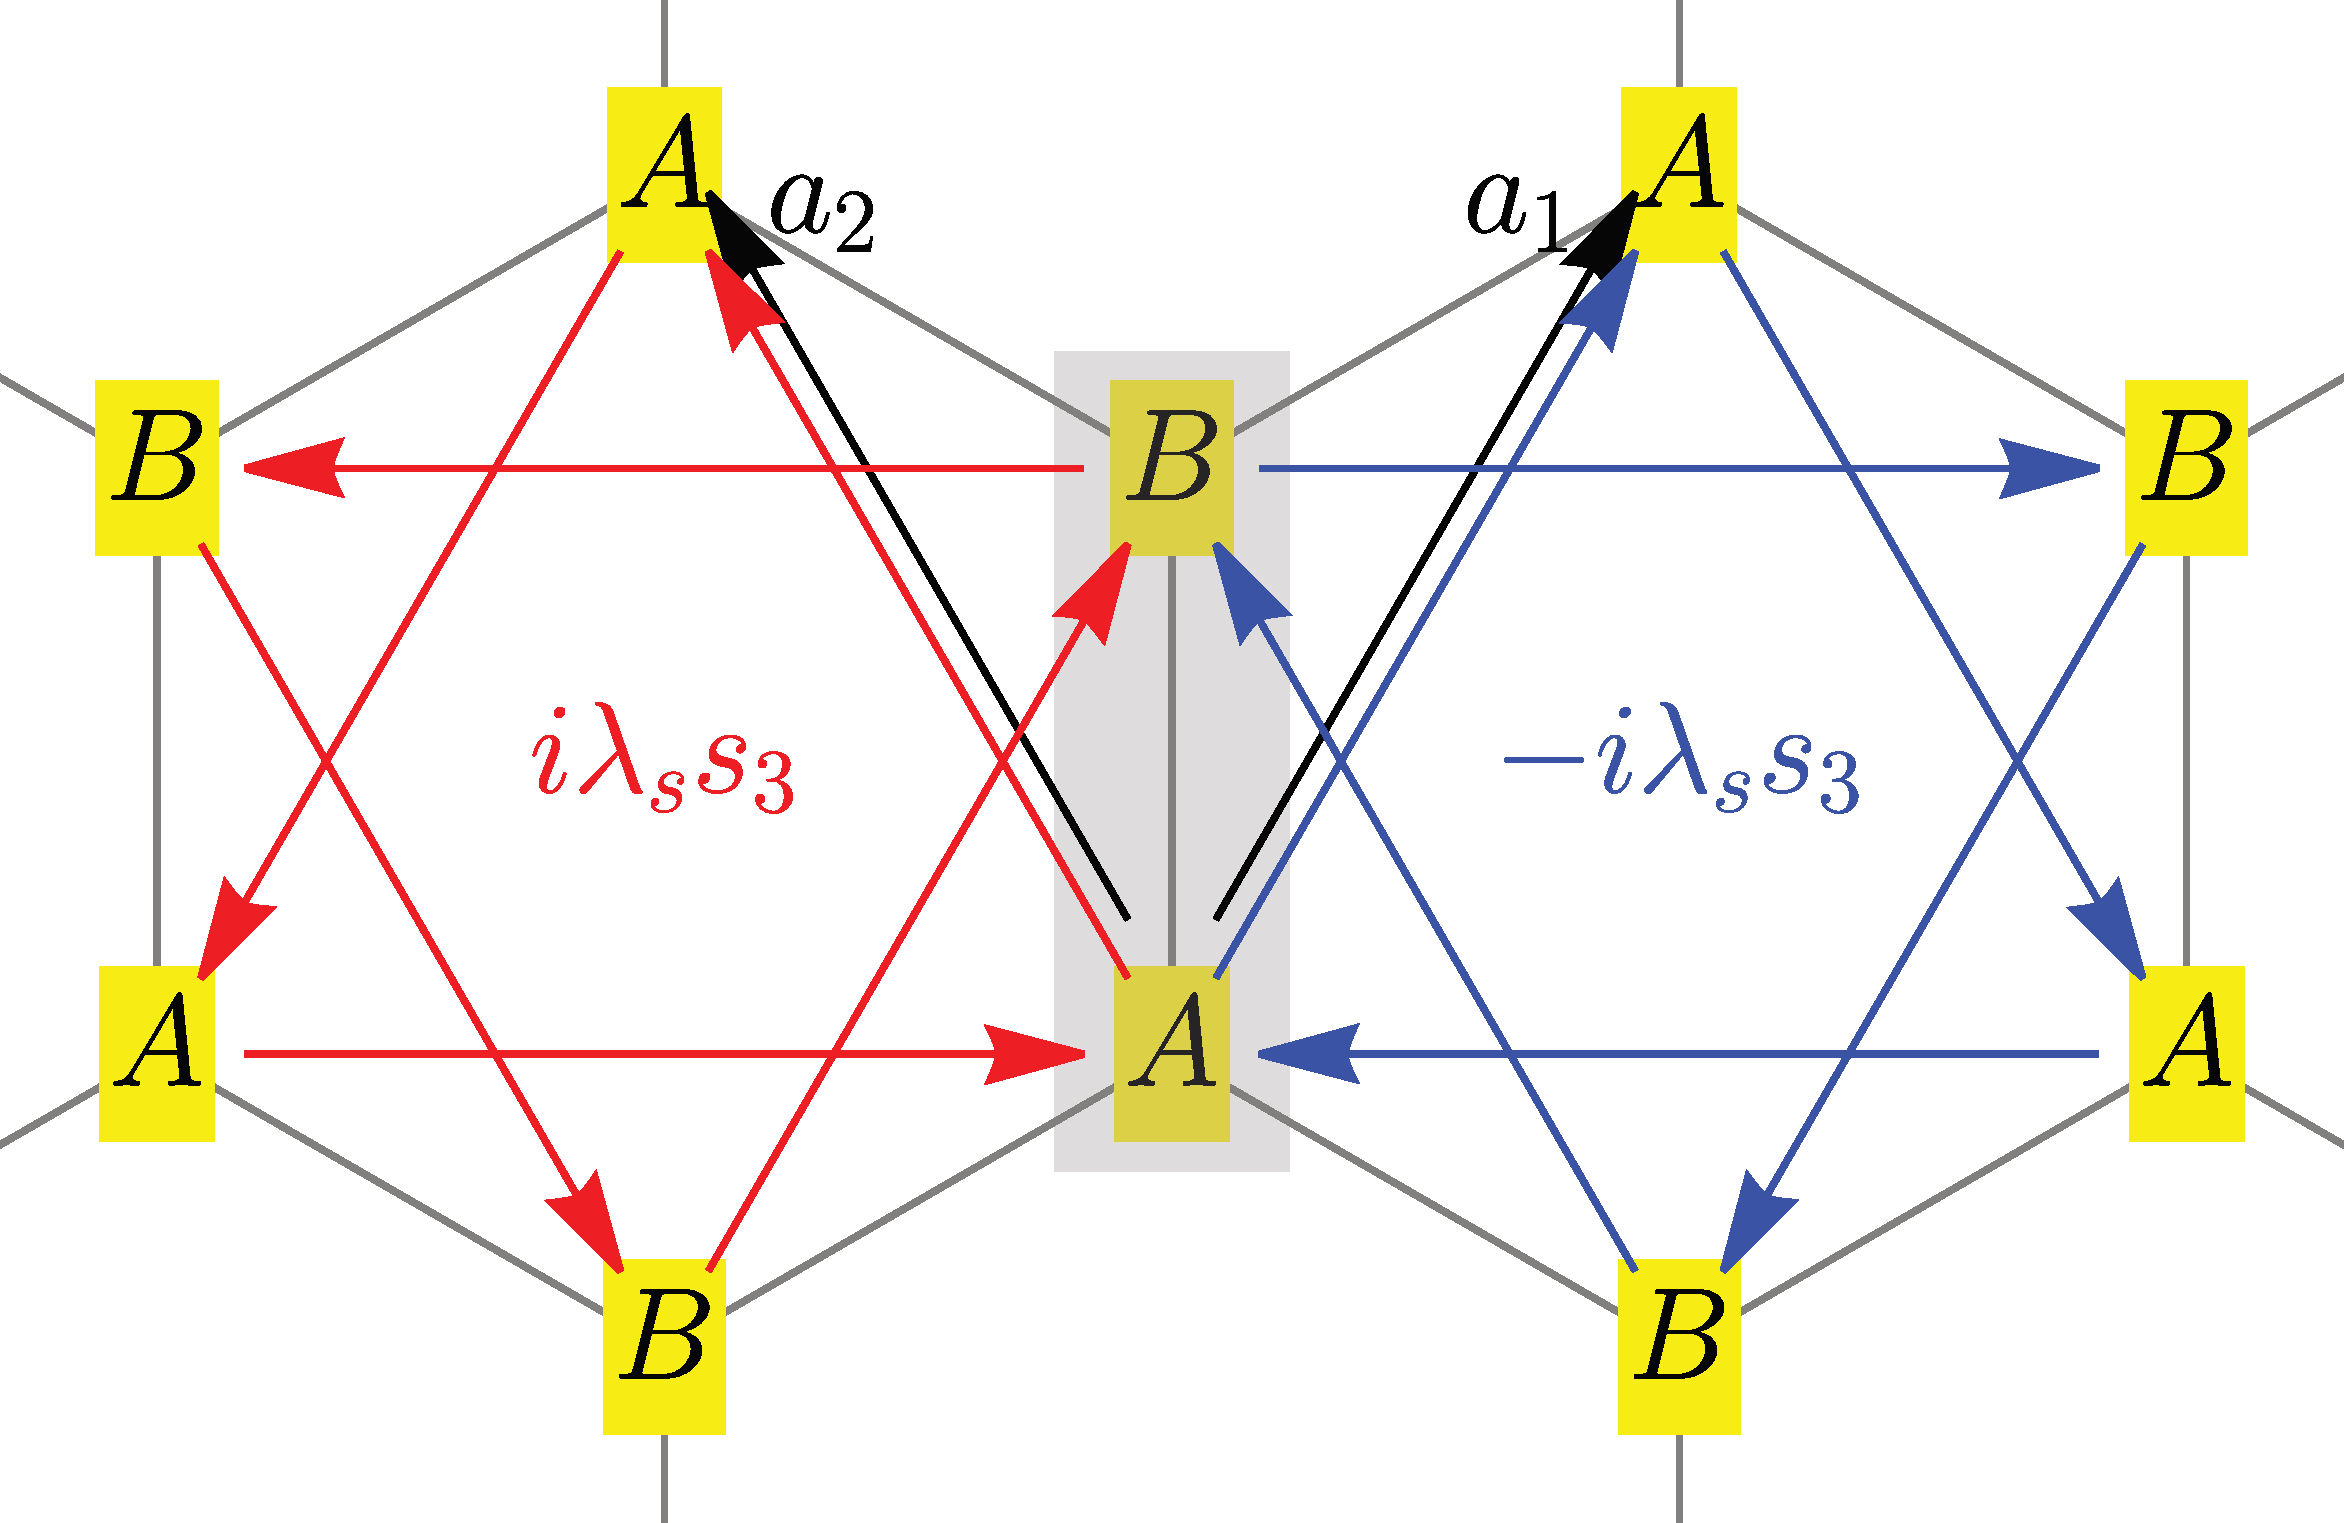
\includegraphics[width=.8\textwidth]{FIGbkmlattice.pdf}
	\caption{KMBH模型在六角晶格上。
	两种子晶格被记为$A$(红)和$B$(蓝),其中一个晶胞被用灰色长方形框出。
	两个黑色向量$\vb a_1$和$\vb a_2$表示Bravais晶格向量。
	次近邻跃迁被用红色和蓝色标出,对于不同赝自旋,这里有一个负号差别。
	这由Pauli矩阵$s_3$暗示,其作用于赝自旋空间。}
	\label{KMBHlattice}
\end{figure}
这里$s_i$($s_0$),$i=1,2,3$,是作用在赝自旋空间的Pauli($2\times 2$单位矩阵)矩阵。
$v_{ij}=\sgn(\vb d_i\times \vb d_j)_z=\pm 1$其中$\vb d_i$和$\vb d_j$是沿着构成次近邻的两个键的向量,
最后一项是一个交替的子晶格势,
它破坏了系统的空间反演对称性。
哈密顿量的相互作用部分是
\begin{equation}
	H_{\tint}= \frac{U}{2}\sum_{j}\sum_{s=\uparrow,\downarrow} a^\dagger_{js}a^\dagger_{js}a_{js} a_{js},\label{hint}
\end{equation}
这里为了简单,我们忽略种间相互作用。



%%%%%%%%%%%%%%%%%%%%%%%%%%%%%%%%%%%%%%%%%%%%%%%%%%%%%%%%%%%%%%%%%%%%%%%%%%%%%%%%%%%%%%%%%%%%%%%%%%%%%%%%%%%%
\begin{figure*}
    \centering
	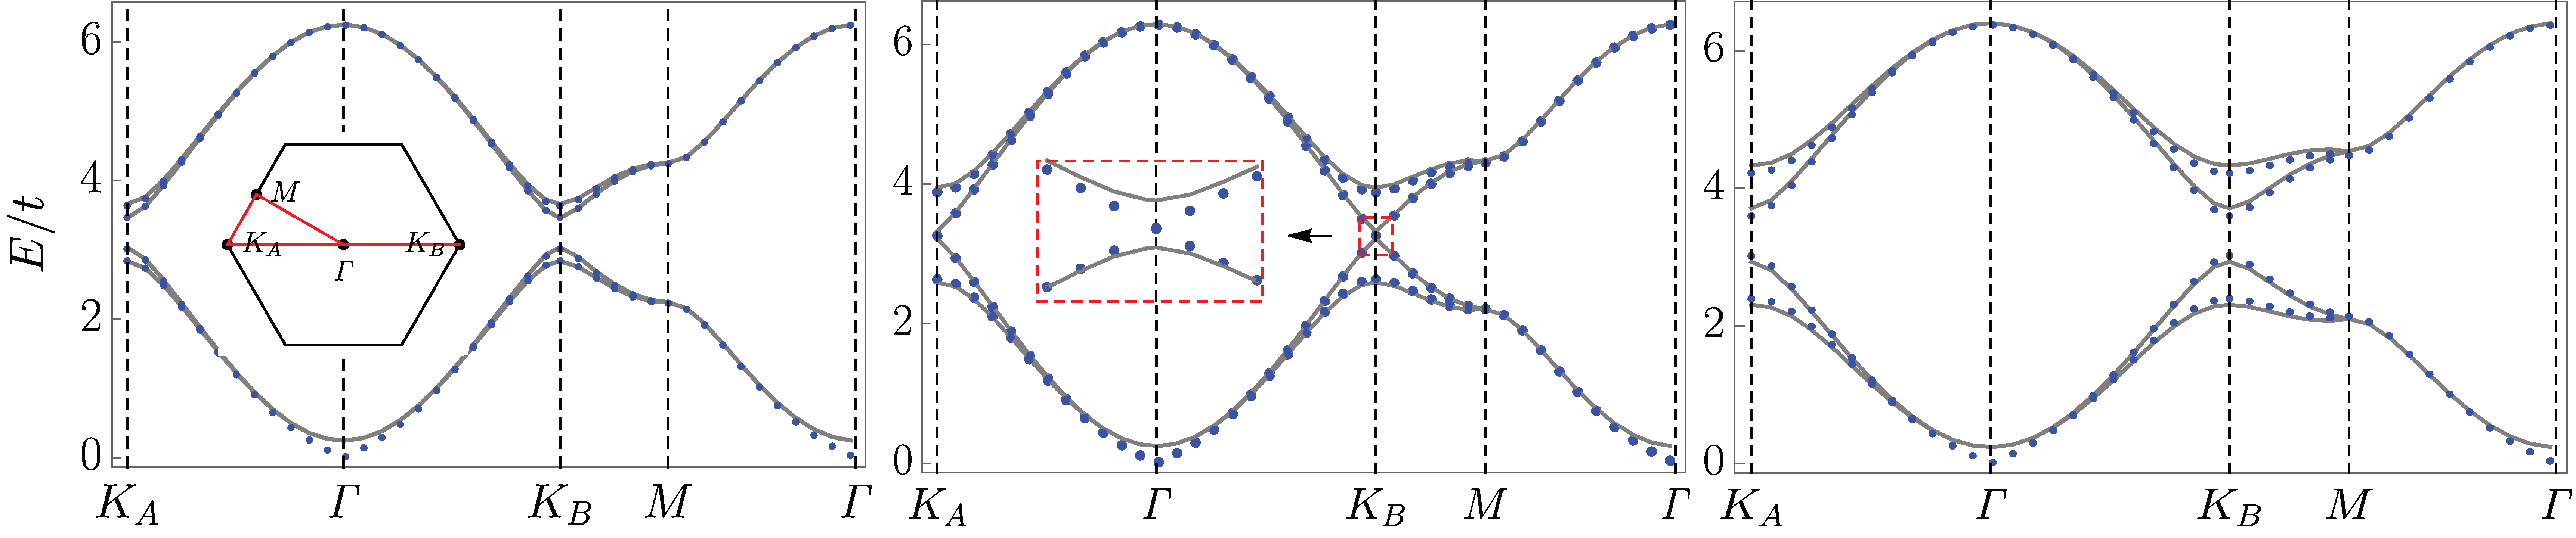
\includegraphics[width=.95\textwidth]{FIGbkmbe.pdf}
	\caption{周期性边界条件下,沿着布里渊区高对称性线(见左图里的嵌入图)的Bogoliubov激发谱,在(左)$\lambda_v/t=0.10$,(中)$\lambda_v/t=\lambda_v^\star/t \approx 0.36$和(右)$\lambda_v/t=0.70$时。无相互作用的能带用灰线标出(向上平移了$nU/2-\mu$)。
	注意当Bogoliubov激发谱的能隙关闭时,
	无相互作用的能隙已经关闭又重新打开了,如中图里的嵌入图所示。
	其他一些参数:$nU/t=1$和$\lambda _s/t=0.06$。}
	\label{KMBHbe}
\end{figure*}
%%%%%%%%%%%%%%%%%%%%%%%%%%%%%%%%%%%%%%%%%%%%%%%%%%%%%%%%%%%%%%%%%%%%%%%%%%%%%%%%%%%%%%%%%%%%%%%%%%%%%%%%%%%%

利用图\ref{KMBHlattice}中所示的Bravais晶格向量,
我们可以把式\eqref{KMBHh0}写在动量空间,
$H_0=\sum_{\vb k}a^\dagger_{\vb k}h(\vb k) a_{\vb k}$,
其中$a_i := (a_{iA\uparrow},a_{iA\downarrow},a_{iB\uparrow},a_{iB\downarrow})^T$,
$4\times 4$的Bloch哈密顿量是
\begin{equation}\label{KMBHh0k}
	h(\vb k)=d_1(\vb k)\Gamma_1+d_2 \Gamma_2+d_{12}(\vb k)\Gamma_{12}+d_{15}(\vb k)\Gamma_{15},
\end{equation}
这里Clifford代数生成元是
\begin{equation}
	\Gamma_a=(\sigma_1 \otimes s_0,\sigma_3 \otimes s_0,\sigma_2\otimes s_1, \sigma_2\otimes s_2,\sigma_2\otimes s_3),\label{gammaKMBH}
\end{equation}
和$\Gamma_{ab}=\frac{1}{2i}[\Gamma_a,\Gamma_b]$,
其中$\sigma_i$ ($\sigma_0$), $i=1,2,3$,是作用在子晶格空间的Pauli矩阵($2\times 2$单位矩阵)。
所有系数列在表\ref{paramtab}中。
在这个表象下,
我们有$\tilde{\mathcal T} \Gamma_a \tilde{\mathcal T}\inv =\Gamma_a$和,
$\tilde{\mathcal T} \Gamma_{ab} \tilde{\mathcal T}\inv =-\Gamma_{ab}$,
其中
\begin{equation}
	\tilde{\mathcal T}=i(\sigma_0\otimes s_2) K = -i\Gamma_{35}K.\label{PTRSop1}
\end{equation}
所以$d_{a}$ ($d_{ab}$) 是关于$\vb k$偶(奇)的,这是由于奇的时间反演对称性:$\tilde{\mathcal T}h(\vb k)\tilde{\mathcal T}\inv = h(-\vb k)$。




%%%%%%%%%%%%%%%%%%%%%%%%%%%%%%%%%%%%%%%%%%%%%%%%%%%%%%%%%%%%%%%%%%%%%%%%%%%%%%%%%%%%%%%%%%%%%%%%%%%%%%%%%%%%
\begin{table}[htb]
    \centering
	\caption{用于式\eqref{KMBHh0k}的参数在前两行给出,额外的用于式\eqref{KMBHheff}的参数在后两行给出,其中$x=\sqrt{3} k_x a/2$和$y=3 k_y a/2$。注意$\bar \theta$是一个关于$\lambda_v/t$和$Un/t$的函数,见图\ref{KMBHtheta}。}
   \label{paramtab}
	\begin{tabular}{cc|cc}
	\hline
		$d_1$ & $-t(1+2\cos x\cos y)$ & $d_2$ & $-\lambda_v$ \\
		\hline
		$d_{12}$ & $2t\cos x\sin y$ & $d_{15}$ & $4\lambda_s(\cos x-\cos y)\sin x$\\
		\hline
		$d_0$ & $\lambda_v\cos \bar \theta+3t\sin \bar \theta+\frac{1}{4}nU\sin^2 \bar \theta$ & $\tilde d_0$ & $\frac{1}{4}nU$ \\
		\hline
		$\tilde d_2$ & $-\lambda_v+\frac{1}{2}nU \cos \bar \theta$ & $\tilde{\tilde{d}}_2$ & $\frac{1}{4}nU \cos \bar \theta$\\
		\hline
	\end{tabular}
\end{table}
%%%%%%%%%%%%%%%%%%%%%%%%%%%%%%%%%%%%%%%%%%%%%%%%%%%%%%%%%%%%%%%%%%%%%%%%%%%%%%%%%%%%%%%%%%%%%%%%%%%%%%%%%%%


%%%%%%%%%%%%%%%%%%%%%%%%%%%%%%%%%%%%%%%%%%%%%%%%%%%%%%%%%%%%%%%%%%%%%%%%%%%%%%%%%%%%%%%%%%%%%%%%%%%%%%%%%%%%
\begin{figure}[th!]
\centering
	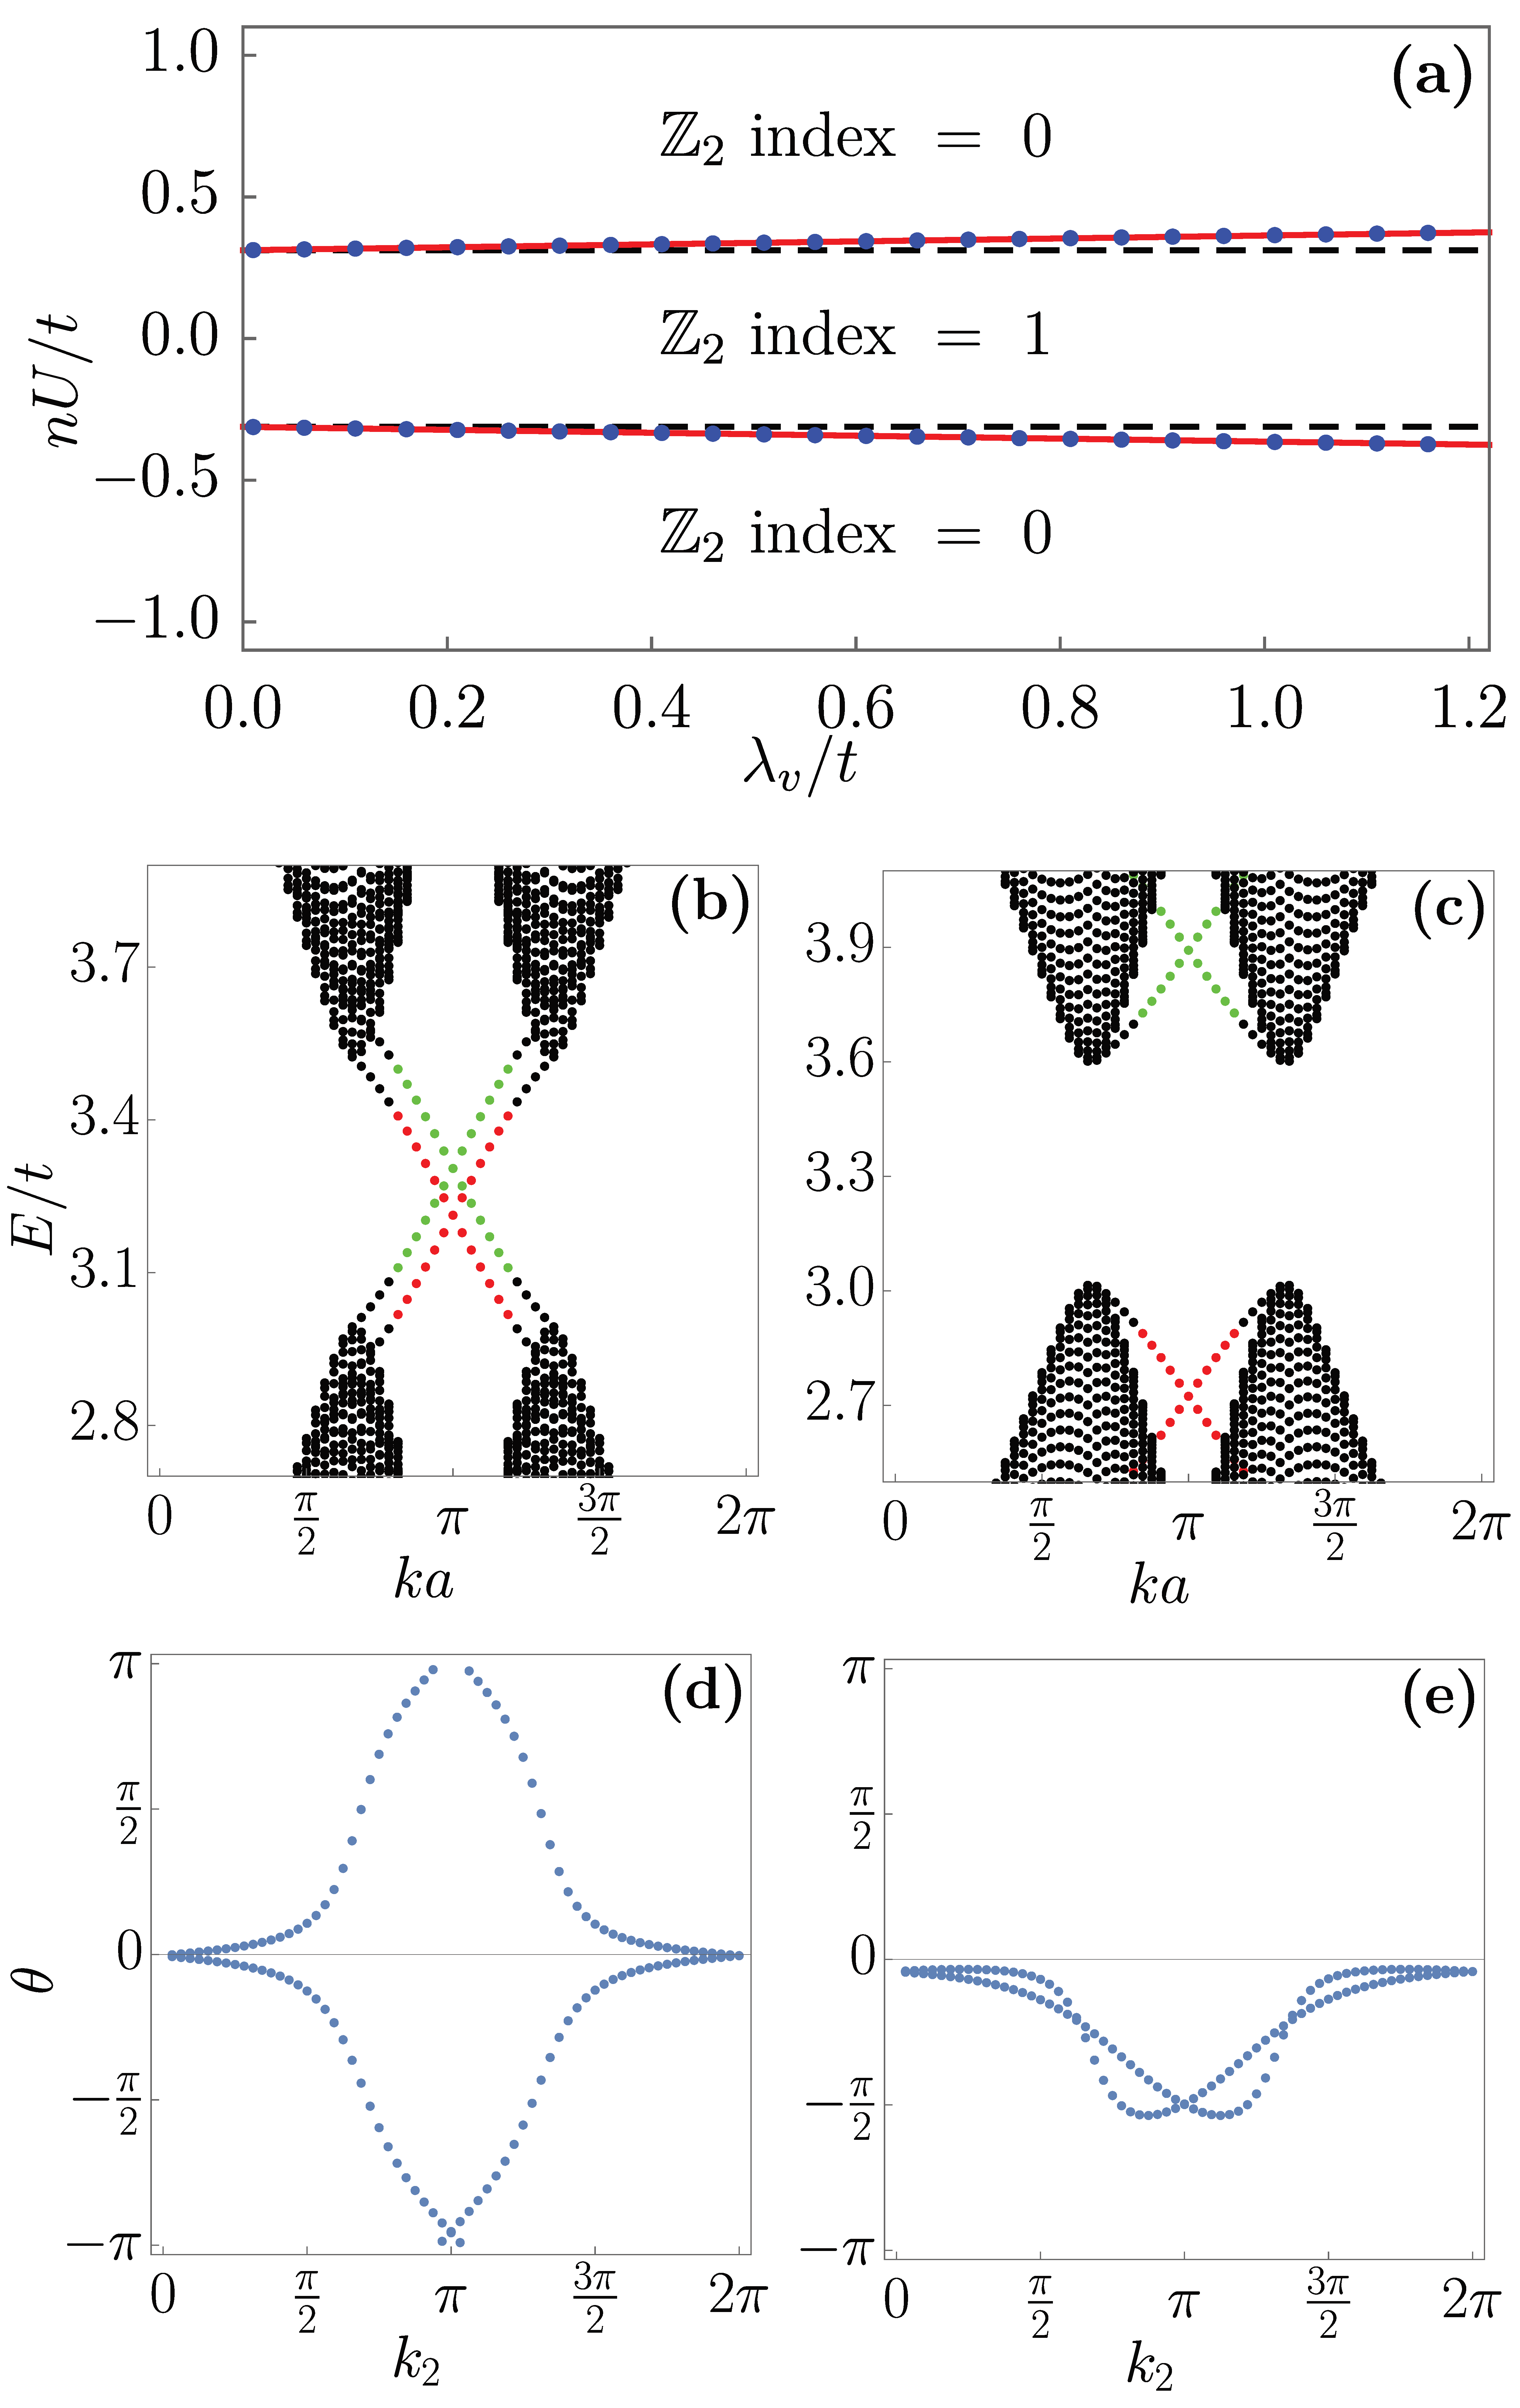
\includegraphics[width=.85\textwidth]{FIGbkmtpd.pdf}
	\caption{\textbf{(a)} 利用式\eqref{fukui}和文献\cite{Fukui2007}给出的数值方法计算的$\mathbb Z_2$不变量,对于最上面的两个能带,在$nU/t=1$和$\lambda_s/t=0.06$时。由蓝点线标出的边界是通过一个完全数值的计算得到的(具体见式\eqref{lv}上面的解释)。红实线是通过一个级数展开得到的,见式\eqref{lv}。
	对比黑色的虚线(对应于无相互作用时的情况),我们发现$\mathbb Z_2$拓扑区域变大了。
	\textbf{(b,c)} Bogoliubov激发谱在一个带状集合上。这里有$64$晶胞,每个包含$64$格点。这里我们使用zigzag边界。
	对于\textbf{(b)},$\lambda_v/t=0.1$;对于\textbf{(c)},$\lambda_z/t=0.7$。
	红(蓝)点对应于边界态,其波函数有大于$80\%$比例在最左(右)的晶胞。注意由于赝时间反演对称性导致的玻色型的Kramers确实存在。\textbf{(d)} and \textbf{(e)} 是最上面两个能带的Wannier中心流动,这里我们把$k_2$当作时间,它们对应于奇的和偶的缠绕数。注意到这里的流动行为是关于$k_2=0$镜面对称的,并且流动是在$k_2=0$和$k_2=\pi$汇合的。这些都和我们在附录给出的证明一致。}
	\label{KMBHtpd}
\end{figure}
%%%%%%%%%%%%%%%%%%%%%%%%%%%%%%%%%%%%%%%%%%%%%%%%%%%%%%%%%%%%%%%%%%%%%%%%%%%%%%%%%%%%%%%%%%%%%%%%%%%%%%%%%%%%

由式\eqref{KMBHh0k}得到的单粒子能带的最小值和Haldane模型\cite{Vasic2015,Furukawa2015}是一样的:
当$\abs{\lambda _s}<t/\sqrt{3}$,
这个最小值在$\vb{\Gamma}$;
对于更大的$\abs{\lambda _s}$,
这个最小值跳到了$\vb K_A$和$\vb K_B$。
这里我们关注前者,该情况下凝聚应该发生在$\vb \Gamma$。
接着,通过写下一个一般的基态波函数并最小化其对应的Gross-Pitaevskii(GP)能量泛函(详见\ref{mfs}),
我们发现超流序参量是$\expval{a_{iA\uparrow}}=\expval{a_{iA\downarrow}}=\cos(\bar \theta/2)\sqrt{n}/2$和$\expval{a_{iB\uparrow}}=\expval{a_{iB\downarrow}}=\sin(\bar \theta/2)\sqrt{n}/2$,
其中$\bar \theta$是一个关于$\lambda_v/t$和$Un/t$的函数(参考图\ref{KMBHtheta})。



通过标准的Bogoliubov理论\ref{mfs},
我们可以得到如下有效哈密顿量
(注意它是非厄米的,因为$\iu$在右边第一行的出现)
\begin{equation}\label{KMBHheff}
	\begin{split}
		H^\eff_{\vb k} &= \tau_0 \otimes [d_{15}(\vb k) \Gamma_{15}] +i \tau_2 \otimes (\tilde d_0 \Gamma_0 + \tilde{\tilde{d}}_2 \Gamma_2)\\
		&\quad + \tau_3 \otimes [d_0\Gamma_0 + d_1(\vb k) \Gamma_1 + \tilde{d}_2 \Gamma_2 + d_{12}(\vb k) \Gamma_{12}]
	\end{split}
\end{equation}
其中$\Gamma_0=\sigma_0\otimes s_0$,所有系数都是实数,并且在表\ref{paramtab}给出。
我们可以发现,这个有效哈密顿量有赝时间反演对称性,其对应的时间反演对称是
\begin{equation}
	\mathcal T= \tau_0\otimes\tilde{\mathcal T}.\nonumber
\end{equation}
通过对角式\eqref{KMBHheff},
我们可以得到Bogoliubov激发谱,如图\ref{KMBHbe}所示。
在低能极限下,这里有两个Goldstone模,这是由于两个$U(1)$对称性破缺导致的,即对应于粒子数和$s_3$守恒。

对于无相互作用哈密顿量,式\eqref{KMBHh0k},
在半满下,系统在有非零的$\lambda_v$时一般是有能隙的。
能隙关闭-打开转变发生在两个角落$\vb K_A$和$\vb K_B$,
当$\lambda_v=\pm 3\sqrt{3}\lambda_s$时 \cite{Kane2005}.
这个行为被Bogoliubov激发谱光滑继承了,唯一的区别是这里$\lambda_v=\lambda_v^\star\neq \pm 3\sqrt{3}\lambda_s$,
如图\ref{KMBHbe}(b)所示。
通过计算$H_{\vb K_A}^\eff$(或者等价的$H_{\vb K_B}^\eff$)的本征值,然后在零第二个和第三个相等(它们被以递减顺序排列),这个临界值$\lambda_v^\star$可以被找到,作为一个关于$\lambda_s$和$nU/t$的函数,我们把它作为蓝线画在了图\ref{KMBHtpd}(a)。
在极限情况$\lambda_s,nU\ll t$下,
我们有
\begin{equation}\label{lv}
	\lambda_v^\star \approx 3\sqrt{3}\lambda _s+\frac{\sqrt{3}}{2}\lambda _s nU/t,
\end{equation}
所以在$U=0$时它这确实回到了无相互作用情况。利用式\eqref{fukui},和Fukui和Hatsugai\cite{Fukui2007}提出的数值计算方法,
对于最上面的两个能带,我们发现$\tilde \Delta_2=1$当$\abs{\lambda_v}<\lambda_v^\star$,
这对应于$\mathbb Z_2$拓扑的区域。
当$\abs{\lambda_v}>\lambda_v^\star$时,$\tilde \Delta_2=0$,
这对应于$\mathbb Z_2$平凡的区域。
我们也计算了对于最上面两个能带的Wannier中心流动,如图\ref{KMBHtpd}(d,e);
以及在一个一维的边界是zigzag型的带状几何上的Bogoliubov激发谱,如图\ref{KMBHtpd}(b,c)。
从而数值地验证了两种$\mathbb Z_2$不变量定义的等价性,
以及体-边对应关系(即螺旋型边界态的出现/消失与$\mathbb Z_2$不变量是拓扑/平凡的有一一对应关系)。

特别地,当$\lambda_v=0$,
我们有$\bar \theta = \pi/2$。
有效哈密顿量这时有一个额外地空间反演对称性,其对应的空间反演对称算符是$\mathcal P=\tau_0\otimes\Gamma_1$。
在四个赝时间反演对称动量处,我们有
\begin{equation*}
	\begin{split}
		(\xi_{00},\xi_{01},\xi_{10},\xi_{11})=(-1,-1,-1,1),
	\end{split}
\end{equation*}
其中$\xi_{ij}$是对于第二对能带在赝时间反演对称动量处$\vb k = i \vb b_1/2 +j \vb b_2/2$的$\mathcal P$算符的本征值。
式\eqref{isz2}暗示$\lambda_v=0$属于$\mathbb Z_2$拓扑的区间,这和之前的讨论一致。

正如式\eqref{lv}(在一个特殊极限下)和图\ref{KMBHtpd}(a)表明的那样,
$\mathbb Z_2$拓扑的区间在随着相互作用(或者平均粒子数)的增加而变大。
为了物理上理解为什么会这样,
首先注意到大$\lambda_v$极限对应于“原子极限”\cite{Bernevig2013},
这时所有原子都紧紧束缚在其中一个子晶格,对应于极端的子晶格失衡,显然是$\mathbb Z_2$平凡的。
所以当从零开始增加$\abs{\lambda_v}$到一个很大的值时
(即从$\mathbb Z_2$拓扑的区间出发),
我们会遇到一个能隙关闭又打开的变化。
另一方面,
排斥相互作用的效果是压制由$\lambda_v$诱导的子晶格的失衡,
因为前者更喜欢一个均匀的构型。
所以,为了达到一个临界的子晶格失衡,我们需要一个更大的$\lambda_v$。

\subsection{Bernevig-Hughes-Zhang-Bose-Hubbard模型}
%%%%%%%%%%%%%%%%%%%%%%%%%%%%%%%%%%%%%%%%%%%%%%%%%%%%%%%%%%%%%%%%%%%%%%%%%%%%%%%%%%%%%%%%%%%%%%%%%%%%%%%%%%%%%
%
%
我们的第二个例子是Bernevig-Hughes-Zhang-Bose-Hubbard(BHZBH)模型。
Bernevig-Hughes-Zhang模型是陈绝缘体的时间反演对称的推广,而后者在冷原子体系中的实验方案被Liu等人提出\cite{Liu2014},
并且已被潘组在实验上实现\cite{Wu_2016,Sun2018}。
所以我们预期BHZBH模型也能很快实验实现。
我们考虑有两种玻色子(用$\eta=A,B$标记),每种又带有一个赝自旋1/2(用$s=\uparrow,\downarrow$标记)。
系统被定义在二维正方晶格,
其无相互作用紧束缚哈密顿量是(见图\ref{bbhzlattice}%
\begin{figure}[th!]
\centering
	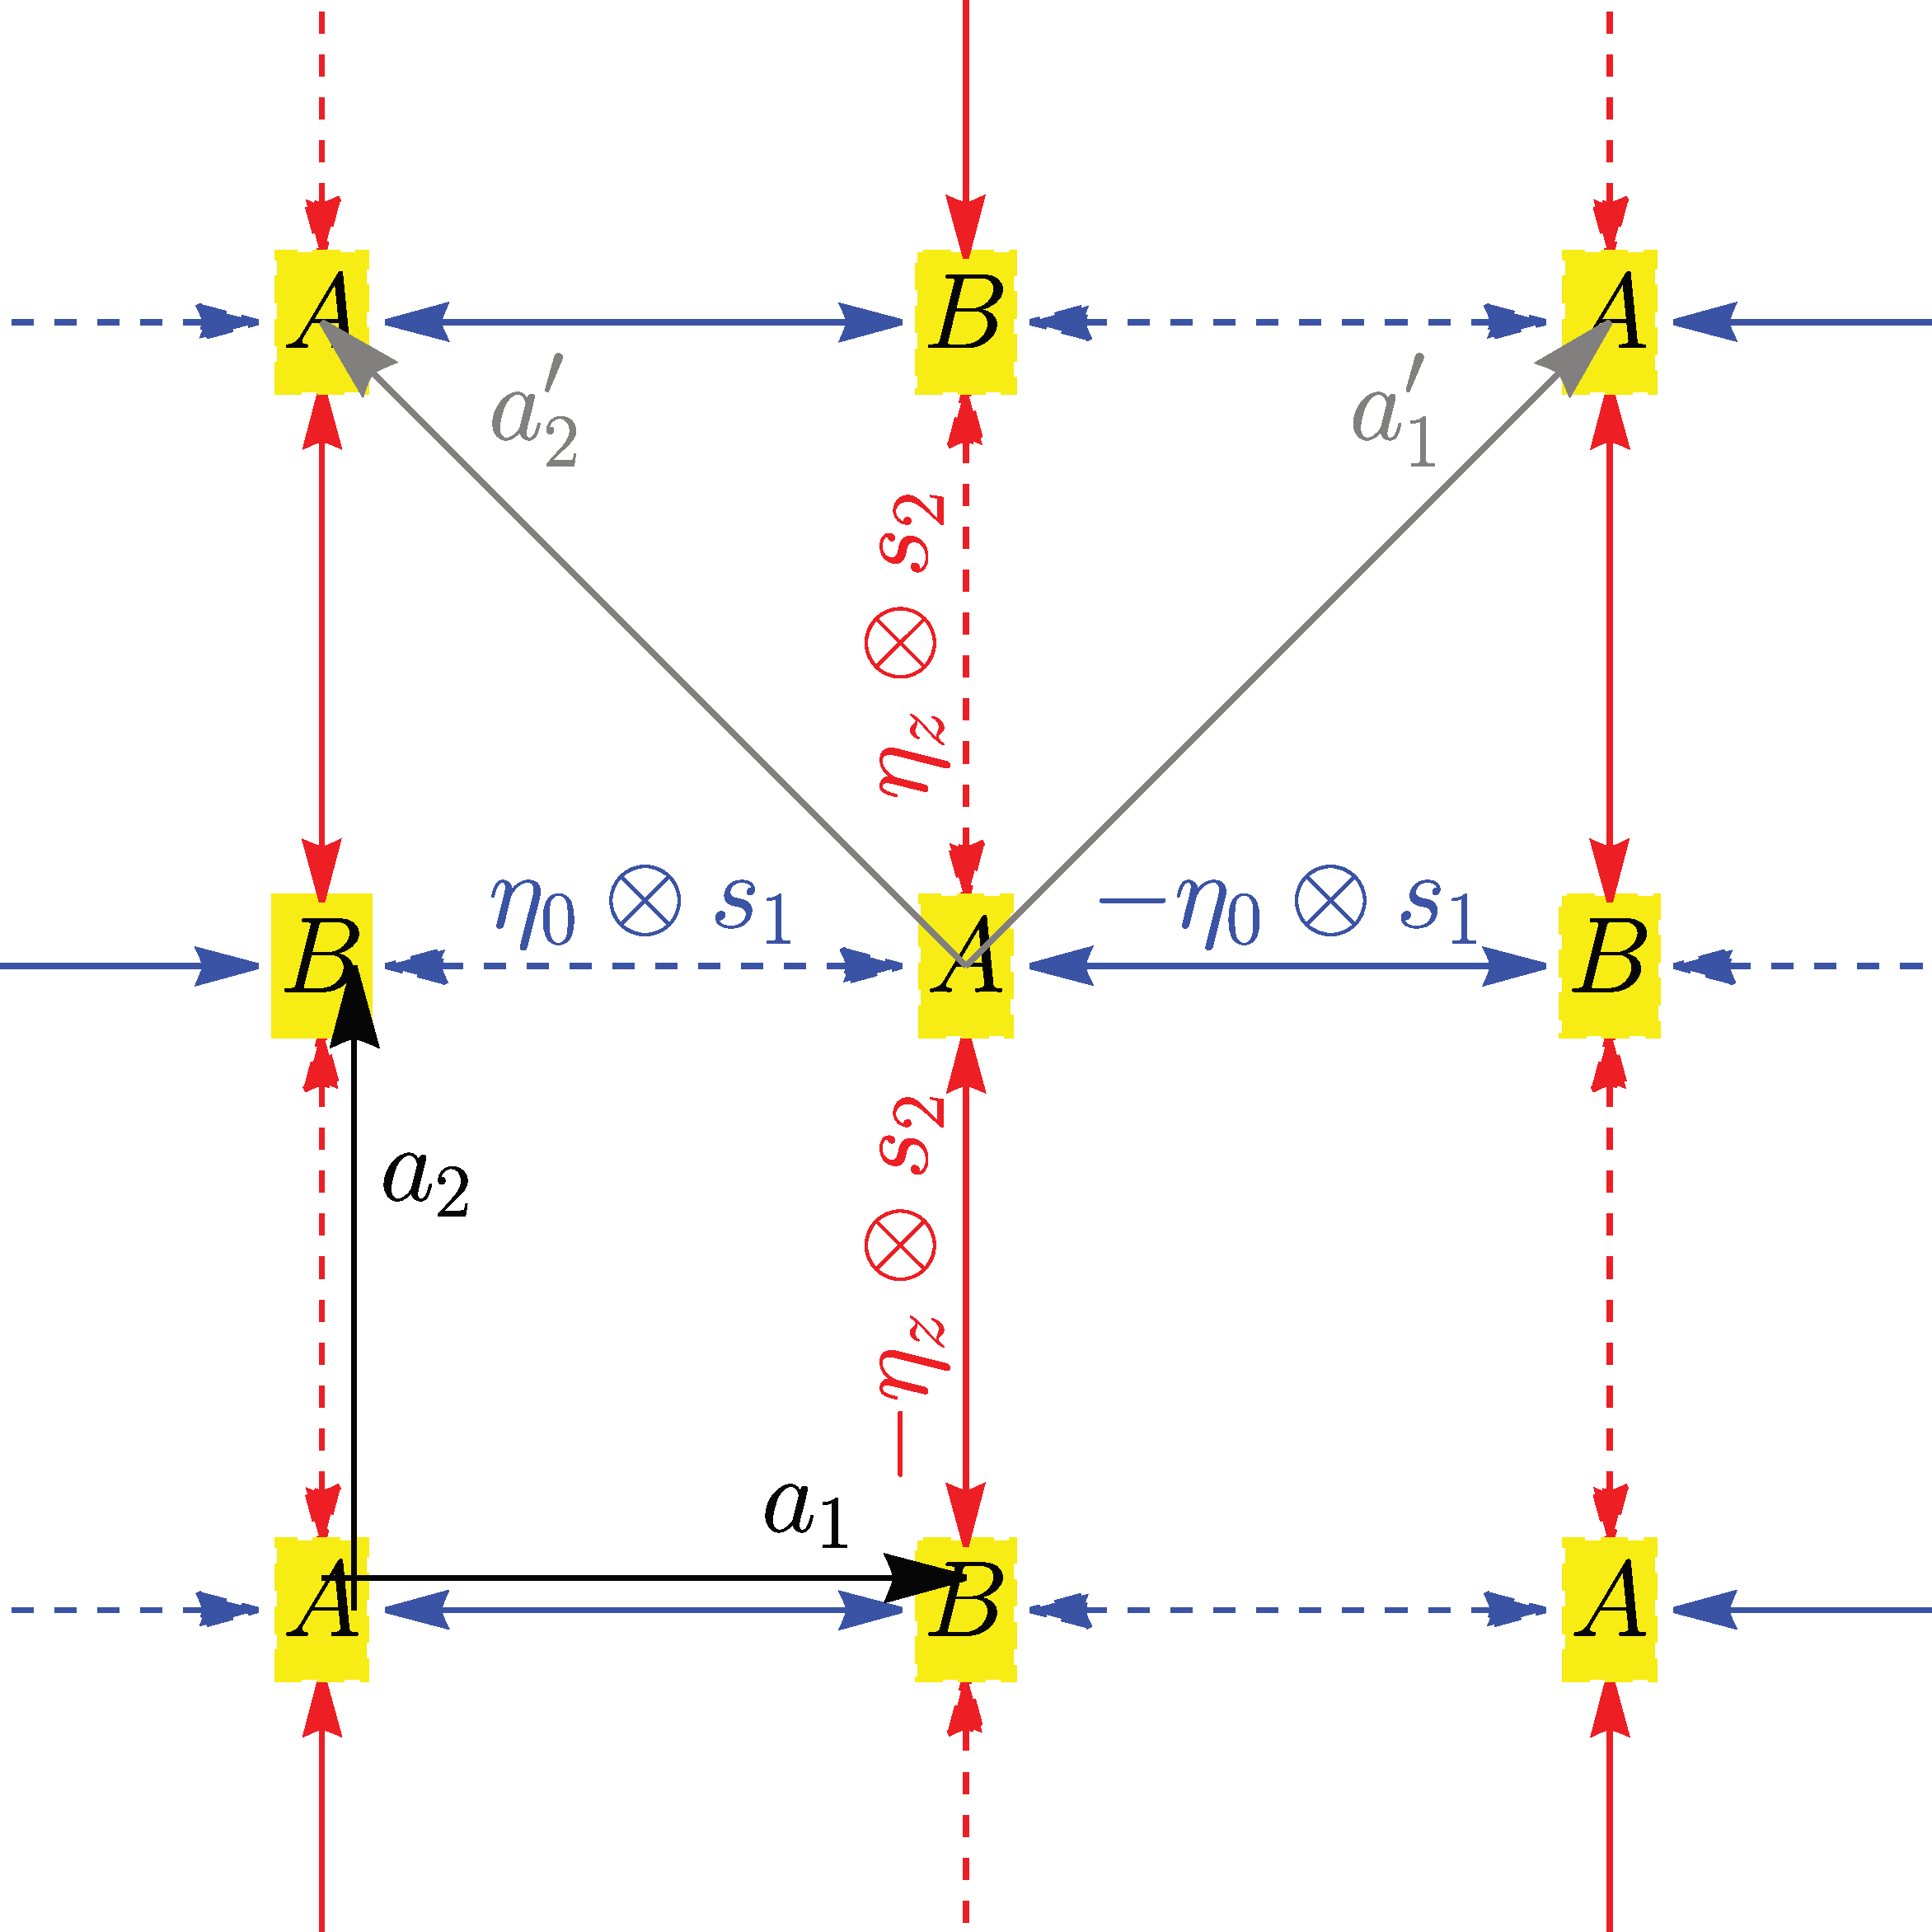
\includegraphics[width=.55\textwidth]{FIGbbhzlattice.pdf}
	\caption{在正方晶格上的BHZBH模型。
	这是刘雄军等人的实验方案的直接推广\cite{Liu2014}。
	式\eqref{bhzorigin}中的,沿x(y)方向的赝自旋翻转的跃迁矩阵$h_s^{ij}$备用蓝色(红色)标出。
	其中箭头表示跃迁方向,
	对同一种颜色,虚线和实线之间相差一个负号。所以在原始的规范下,每个晶胞包含两个子晶格,其对应的Bravais原初晶格向量$\vb a_{1,2}'$由灰色标出\cite{Lang2017}。
	在经过一个规范变换$a_{j\eta\downarrow}\rightarrow (-1)^{j}a_{j\eta\downarrow}$ \cite{Liu2014}后,
	所有的线都变成实线,
	然后我们可以用红线标出的$\vb a_{1,2}$作为Bravais格点向量,对应的晶胞只包含一个格点。}
	\label{bbhzlattice}
\end{figure}
),
\begin{equation}\label{bhzorigin}
\begin{split}
	H_0 &=-t\sum_{\expval{i,j}}a^\dagger_i (\eta_0\otimes s_0) a_j-m_z\sum_i a^\dagger_i (\eta_0\otimes s_3) a_i  \\
	&\quad -t_s \sum_{\expval{i,j}} a^\dagger_i h_s^{ij} a_j,
\end{split}
\end{equation}
这里$a_{i\eta s}^{(\dagger)}$是在格点$\vb r_i$的第$\eta$种赝自旋为$s$玻色子的湮灭(产生)算符,
并且我们定义$a_i := (a_{iA\uparrow},a_{iA\downarrow},a_{iB\uparrow},a_{iB\downarrow})^T$。
$\eta_i$ ($\eta_0$)和$s_i$ ($s_0$), $i=1,2,3$, 是Pauli矩阵($2\times 2$单位矩阵)分别作用在两种玻色子和赝自旋空间的。$t$是赝自旋守恒的跃迁,$m_z$是一个Zeeman项。
赝自旋翻转的跃迁矩阵$h_s^{ij}$如图\ref{bbhzlattice}所示。
注意$\eta_3$的出现,它暗示两种玻色子沿$x$方向跃迁的系数相差一个符号。这直接导致了式\eqref{bhzorigin}存在奇的时间反演对称性\cite{Asboth2016}。
我们假设对于每种玻色子,哈密顿量的相互作用部分和式\eqref{hint}相同。

通过一个规范变换$a_{j\eta\downarrow}\rightarrow (-1)^{j}a_{j\eta\downarrow}$ \cite{Liu2014},
动量空间的Bloch哈密顿量是
\begin{equation}\label{hkbhz}
\begin{split}
		h(\vb k)&=\eta_0\otimes\big\{[-2t(\cos k_x+\cos k_y)-m_z] s_3\\
	&\quad -2t_s \sin k_x s_2\}+\eta_3\otimes(-2t_s \sin k_y s_1),
\end{split}
\end{equation}
它类似由Bernevig, Hughes and Zhang提出的HgTe的4-带模型,
这个单粒子哈密顿量有奇的时间反演对称性,其对应的时间反演算符是
\begin{equation}
	\tilde{\mathcal T}h(\vb k)\tilde{\mathcal T}\inv =h(-\vb k),\quad \tilde{\mathcal T}=i\eta_2\otimes s_0 K,\nonumber
\end{equation}
它也有空间反演对称性,其对应的空间反演算符是
\begin{equation}
	\tilde{\mathcal P}h(\vb k)\tilde{\mathcal P}\inv =h(-\vb k),\quad \tilde{\mathcal P}=\eta_0\otimes s_3.\nonumber
\end{equation}

这里区分于式\eqref{gammabkm},我们选择让Dirac矩阵在$\tilde{\mathcal P}\tilde{\mathcal T}$作用下是偶的 \cite{Fu2007},
\begin{equation*}
	\Gamma_a=\pqty{\eta_0\otimes s_3,\eta_0\otimes s_2,\eta_1\otimes s_1,\eta_2\otimes s_1,\eta_3\otimes s_1}.
\end{equation*}
所以$\tilde{\mathcal T}=-i\Gamma_{35}K$,$\tilde{\mathcal P}= \Gamma_1$,
以及对易子在$\tilde{\mathcal P}\tilde{\mathcal T}$的作用下是奇的,
即$\tilde{\mathcal P}\tilde{\mathcal T}\Gamma_{ab}(\tilde{\mathcal P}\tilde{\mathcal T})\inv=-\Gamma_{ab}$。
由于$\Gamma_1=\tilde{\mathcal P}$,我们还有
\begin{equation}
	\tilde{\mathcal T} \Gamma_a\tilde{\mathcal T}= \tilde{\mathcal P}\Gamma_a\tilde{\mathcal P}=\begin{cases}
		&+\Gamma_a \qfor a=1,\\
		&-\Gamma_a \qfor a\neq 1.
	\end{cases}\nonumber
\end{equation}
式\eqref{hkbhz}于是变为
\begin{equation}\label{hkbhz1}
	h(\vb k)=d_1(\vb k)\Gamma_1+d_{2}(\vb k)\Gamma_{2}+d_{5}(\vb k)\Gamma_{5},
\end{equation}
其中所有系数都是实数,并且在表\ref{paramtabBHZ}中列出。
如文献\cite{Fu2007}给出,这个无相互作用模型的$\mathbb Z_2$不变量可以通过式\eqref{isz2}求得。
这里的Dirac矩阵的表象已被取成使得在四个时间反演不变动量处,只有系数$d_1$是可能非零的。
即$h(\vb \Lambda )=d_1(\vb \Lambda )\tilde{\mathcal P}$。
所以我们可以很容易得到所有占据态的$\tilde{\mathcal P}$的本征值,
\begin{equation}
	(\xi_{00},\xi_{01},\xi_{10},\xi_{11})=(-4t-m_z,-m_z,-m_z,4t-m_z),\label{nonBHZis}
\end{equation}
上式暗示了无相互作用系统在$\abs{m_z}<4t$时处于$\mathbb Z_2$拓扑相,而其他情况下处于$\mathbb Z_2$平凡相。


%%%%%%%%%%%%%%%%%%%%%%%%%%%%%%%%%%%%%%%%%%%%%%%%%%%%%%%%%%%%%%%%%%%%%%%%%%%%%%%%%%%%%%%%%%%%%%%%%%%%%%%%%%%%%

%%%%%%%%%%%%%%%%%%%%%%%%%%%%%%%%%%%%%%%%%%%%%%%%%%%%%%%%%%%%%%%%%%%%%%%%%%%%%%%%%%%%%%%%%%%%%%%%%%%%%%%%%%%%%



%%%%%%%%%%%%%%%%%%%%%%%%%%%%%%%%%%%%%%%%%%%%%%%%%%%%%%%%%%%%%%%%%%%%%%%%%%%%%%%%%%%%%%%%%%%%%%%%%%%%%%%%%%%%%
\begin{table}[htb]
    \centering
	\caption{前两行展示了被用在式\eqref{hkbhz1}的系数;额外的用在式\eqref{bbhzheff}中的系数被展示在后两行。}
   \label{paramtabBHZ}
	\begin{tabular}{cc|cc}
	\toprule
		$d_1$ & $-2t(\cos k_x +\cos k_y)-m_z$ & $d_{2}$ & $-2t_s\sin k_x$ \\
		\hline
		$d_{5}$ & $-2t_s \sin k_y$ & \\
		\midrule
		$\tilde d_1$ & $\frac{nU}{2}+d_1$ & $d_0$ & $\frac{nU}{4}$ \\
		\hline
		$\tilde d_0$ & $4t+m_z$ &  & \\
		\bottomrule
	\end{tabular}
\end{table}
%%%%%%%%%%%%%%%%%%%%%%%%%%%%%%%%%%%%%%%%%%%%%%%%%%%%%%%%%%%%%%%%%%%%%%%%%%%%%%%%%%%%%%%%%%%%%%%%%%%%%%%%%%%%%

式\eqref{hkbhz}给出的单粒子能带和陈绝缘体的一样,只是由于有$\tilde{\mathcal P}\tilde{\mathcal T}$对称性,所以有两重简并。对于$\abs{t_s}<t_s^\star$,其中$t_s^\star=\sqrt{2t^2+m_z t/2}$,能带最小值在$\vb \Gamma$ ($\vb M$) 如果 $m_z>0$ ($m_z<0$)。对于$\abs{t_s}>t_s^\star$,
这个单一最小值分裂成4个点,$(\pm k_0,\pm k_0)$,其中$k_0=\arccos\frac{m_z t}{2(t_s^2 -2t^2)}$。
这里我们只关注前者,并且假设玻色子只凝聚在$\vb \Gamma$,
这个假设总可以通过添加一个足够大的$m_z$达到。
然后通过考虑一个一般的基态波函数ansatz,并且最小化对应的GP能量泛函(详见\ref{mfs}),我们得到超流序参量$\expval{a_{iA\uparrow}}=\expval{a_{iB\uparrow}}=1/\sqrt{2}$ and $\expval{a_{iA\downarrow}}=\expval{a_{iB\downarrow}}=0$(见图\ref{bbhztheta})。

利用Bogoliubov理论,我们得到有效哈密顿量(注意由于右边第一行$\iu$的出现,这个哈密顿量是非厄米的)\ref{mfs},
\begin{equation}\label{bbhzheff}
	\begin{split}
		H_{\vb k}^\eff &= d_{5}\tau_0\otimes\Gamma_{5} +id_0 \tau_2\otimes(\Gamma_0+\Gamma_1)\\
		&\quad \tau_3\otimes(\tilde{d}_0 \Gamma_0 + \tilde{d}_1 \Gamma_1 + d_2 \Gamma_{2}),
	\end{split}
\end{equation}
其中$\Gamma_0=\eta_0\otimes s_0$,所有系数都是实数,并且在表\ref{paramtabBHZ}中给出。
容易发现,这个有效哈密顿量同时有赝时间反演对称性和空间反演对称性。前者对应的算符是
\begin{equation}
	\mathcal T=\tau_0\otimes\tilde{\mathcal T},\label{PTRSop2}
\end{equation}
而后者对应的算符是
\begin{equation}
	\mathcal P=\tau_0\otimes\tilde{\mathcal P}.\label{ISop}
\end{equation}
通过对角式\eqref{bbhzheff},我们可以得到Bogoliubov激发谱,如图\ref{bbhzbe}%
\begin{figure*}[th!]
\centering
	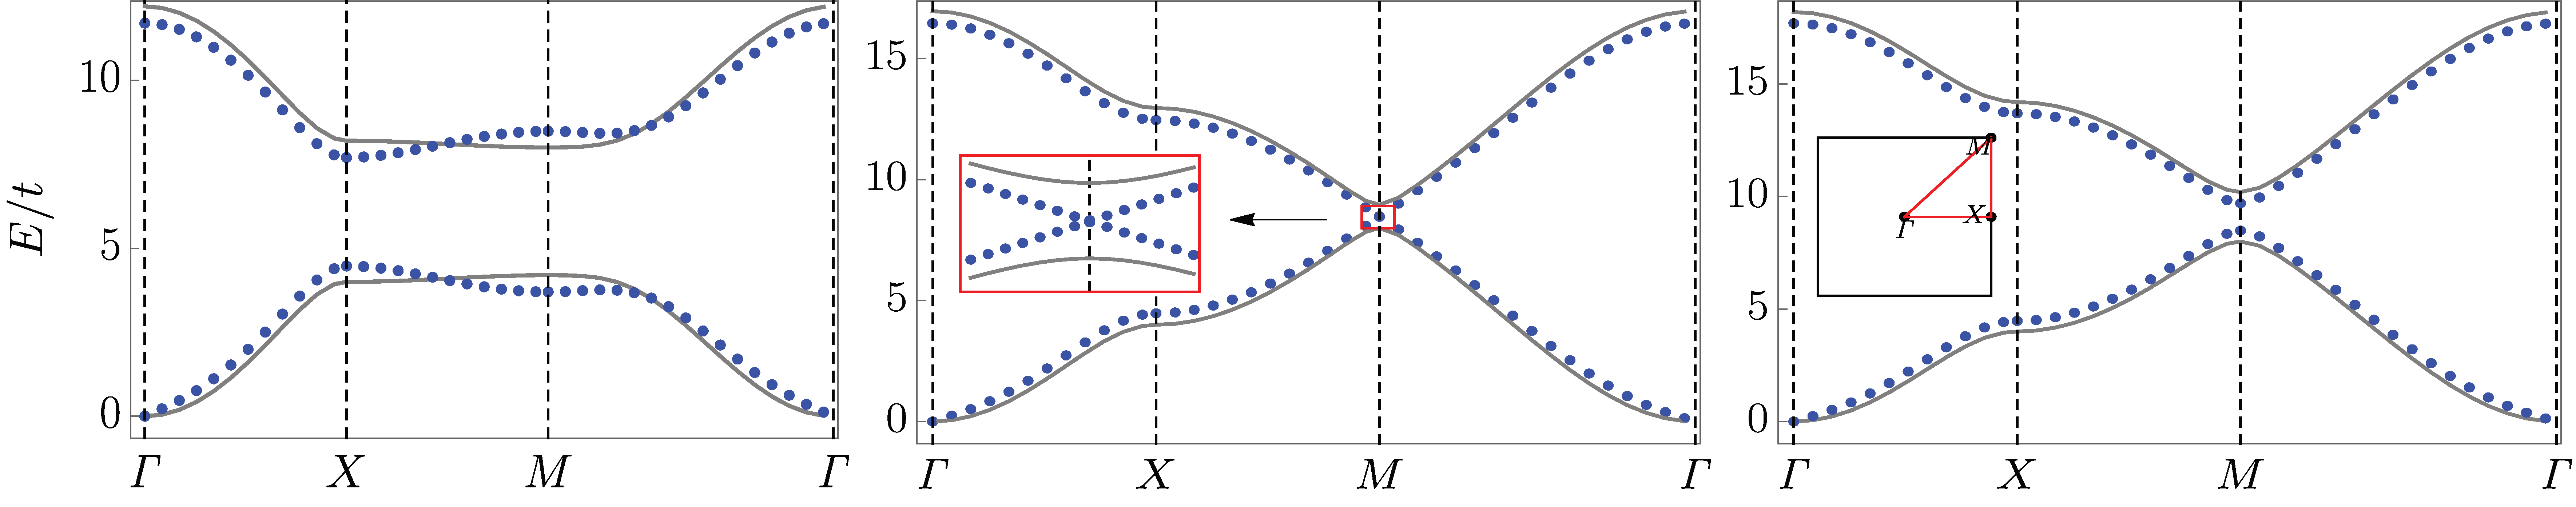
\includegraphics[width=.95\textwidth]{FIGbbhzbe.pdf}
	\caption{在周期边界条件下,沿着第一布里渊区高对称点(见右图的嵌入图)的Bogoliubov激发谱(蓝点)。左$m_z/t=2.10$,中$m_z/t=m_z^\star/t\approx 4.48$,右$m_z/t=5.10$。
	无相互作用能带(往上移了$nU/2-\mu$) 被用灰色实线标出。
	注意到当Bogoliubov能带能隙关闭时,对应的无相互作用能带已经关闭又重打开了(见中图)。其他相关参数:$nU/t=t_s/t=1$.}
	\label{bbhzbe}
\end{figure*}
所示。这里有一个两重简并,是由于$\mathcal P\mathcal T$对称性。
在低能极限下,
这里有两支Goldstone模,这是由于基态自发对称破缺了系统的两个连续对称性,分别对应于粒子数守恒和$\eta_3$守恒。

%%%%%%%%%%%%%%%%%%%%%%%%%%%%%%%%%%%%%%%%%%%%%%%%%%%%%%%%%%%%%%%%%%%%%%%%%%%%%%%%%%%%%%%%%%%%%%%%%%%%%%%%%%%%

%%%%%%%%%%%%%%%%%%%%%%%%%%%%%%%%%%%%%%%%%%%%%%%%%%%%%%%%%%%%%%%%%%%%%%%%%%%%%%%%%%%%%%%%%%%%%%%%%%%%%%%%%%%%

对于无相互作用的哈密顿量式\eqref{hkbhz1},
如果$m_z$是正的,能隙的关闭再打开转变点发生在$\vb M$,当$m_z=4t$时(参考式\eqref{nonBHZis})。
这个行为被Bogoliubov激发谱光滑地继承了,除了现在转变点发生在$m_z=m_z^\star\neq4t$,
如图\ref{bbhzbe}(b)所示。通过计算$H_{\vb M}^\eff$的本征值,并且令相关的两个相等,我们发现
\begin{equation}\label{lzc}
	m_z^\star= \sqrt{2t(8t+nU)}+\frac{nU}{4},
\end{equation}
所以当令$U=0$时,我们的确回到了无相互作用情况。
利用式\eqref{fukui},以及Fukui和Hatsugai的数值方法\cite{Fukui2007},
对于粒子能带的最上面一对能带,我们发现当$m_z<m_z^\star$时,$\tilde \Delta_2=1$,即对应于$\mathbb Z_2$拓扑的区域;
而当$m_z>m_z^\star$时,$\tilde \Delta_2=0$,
即对应于$\mathbb Z_2$平凡的区域。
我们也计算了最上面一对能带的Wannier中心流动,以及在一个带状几何上的Bogoliubov激发谱,见图\ref{bbhztpd}。%
\begin{figure}[th!]
\centering
	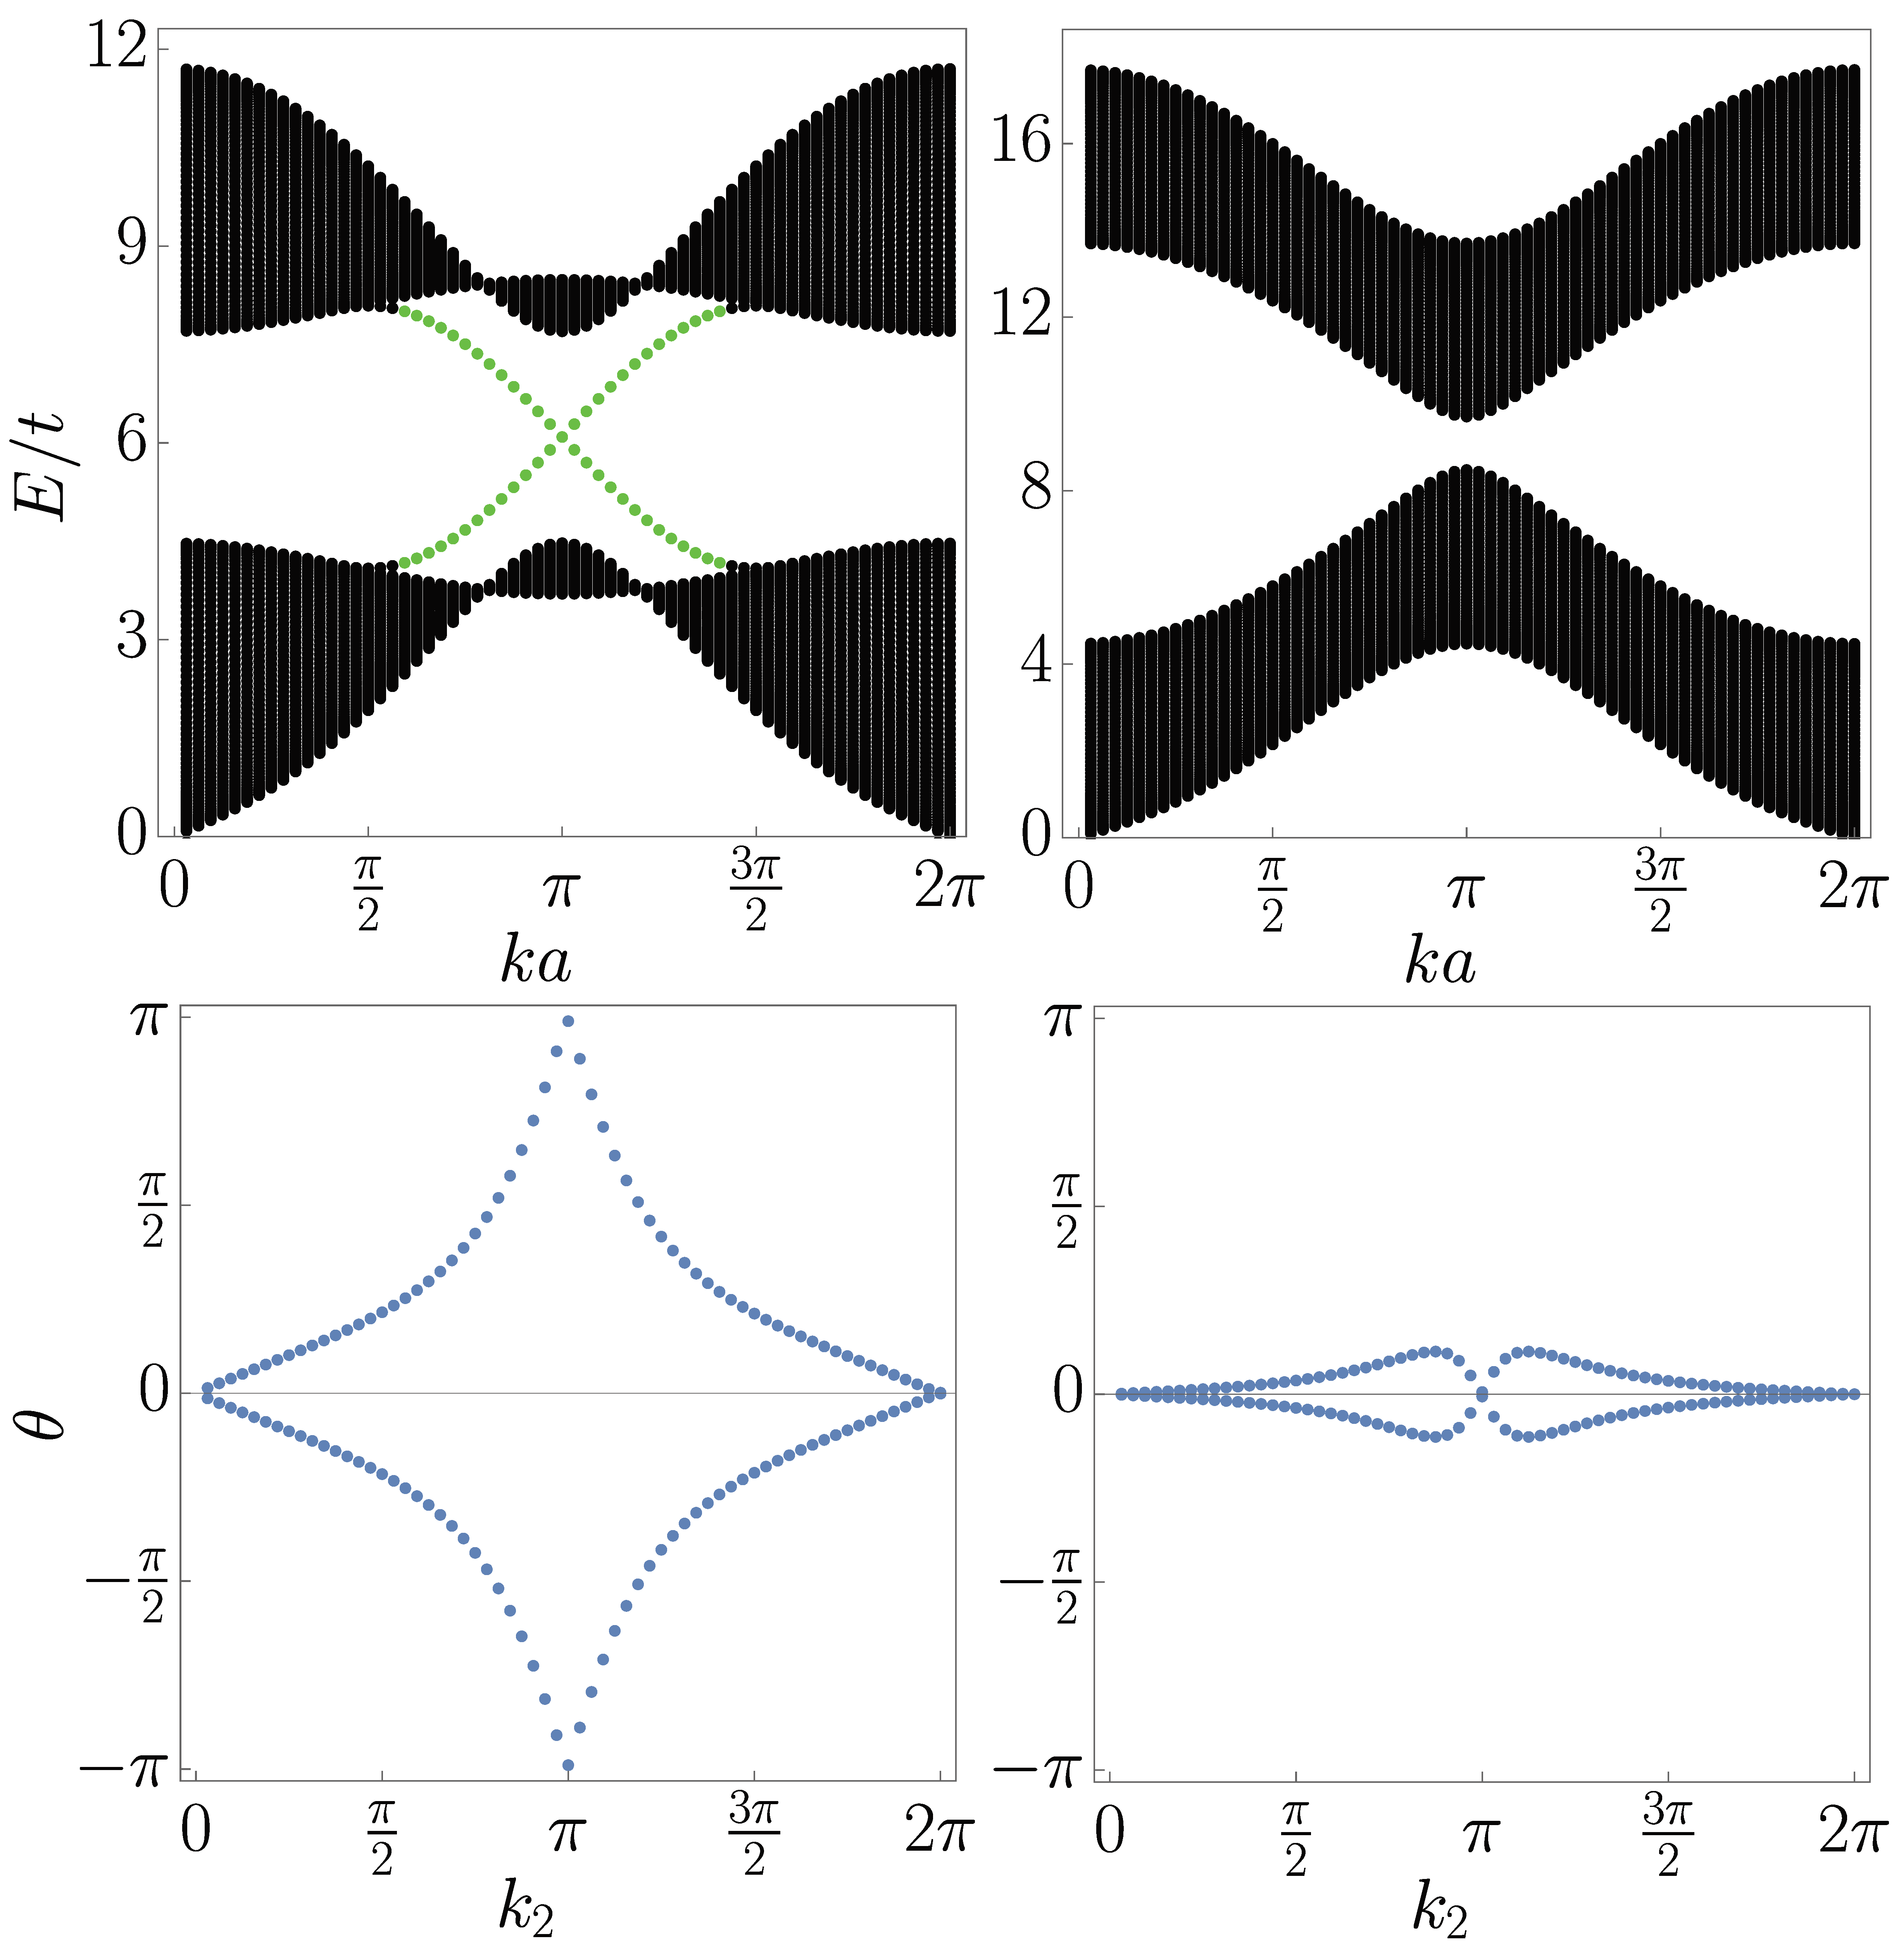
\includegraphics[width=.95\textwidth]{FIGbbhztpd.pdf}
	\caption{上两图:在带状几何下的Bogoliubov激发谱,这里每个晶胞包含了64个格点。左:$m_z/t=2.1$,右:$m_z/t=5.1$。绿点对应与边界态,它的波函数有大于$80\%$的比例在最右边。在左边的边界态由于空间反演对称性,和绿点完全重合。下两图:对应于上图的,上面一对能带的Wannier中心流动,其中我们把$k_2$看作时间,它们分别有奇数和偶数的缠绕。注意这个流动行为是关于$k_2=0$面对称的,并且它们在$k_2=0$和$k_2=\pi$汇合。额外地,由于空间反演对称性,Wannier中心流动也是关于$\theta=0$面对称的。其他参数:$nU/t=t_s/t=1$。}
	\label{bbhztpd}
\end{figure}
这些结果验证了两种定义$\mathbb Z_2$不变量方式的等价性,以及体-边对应的正确性。

由于这个系统有空间反演对称性,我们也可以通过检查空间反演算符在赝时间反演不变动量处的本征值来确定能带是否时拓扑的。
由于能隙只在$\vb M$关闭,本征值的变化只可能在此处发生。所以我们只考虑两个相关的能带在$\vb M$的本征值:(注意对于$l=1,2$,$E_{l+1}=E_l$),
\begin{equation*}
	\begin{split}
		E_1(\vb M) &=\sqrt{8t(8t+nU)},\qquad E_3(\vb M)=2m_z-\frac{nU}{2}, \\
		\ket{u_1(\vb M)} &\propto (0,0,-\frac{16t + nU +4\sqrt{2t(8t+nU)}}{nU},0,0,0,1,0)^T, \\ \ket{u_3(\vb M)} &= (0,0,0,1,0,0,0,0)^T.
	\end{split}
\end{equation*}
这些本征向量同样也是空间反演算符的本征向量,对应的本征值分别是$1$和$-1$。
所以拓扑转变发生在能量简并时,$E_1(\vb M)=E_3(\vb M)$,
从而导出式\eqref{lzc}。
为了确定螺旋型边界态的存在与否,我们必须检查$\mathcal P$在所有四个赝时间反演不变动量处的本征值,
\begin{equation*}
	(\xi_{00},\xi_{01},\xi_{10},\xi_{11})=(-1,1,1,1),\qfor m_z<m_z^\star.
\end{equation*}
由此,我们根据式\eqref{isz2}得知$m_z<m_z^\star$对应于$\mathbb Z_2$拓扑的能带,而$m_z>m_z^\star$对应于$\mathbb Z_2$平凡的能带。

最后我们注意到$\mathbb Z_2$拓扑的区域在BHZBH模型中也随着相互作用(或者粒子数密度)的增加变大了,如式\eqref{lzc}所示。
和KMBH模型类似,物理地说,这个排斥性的相互作用更喜欢一个均匀的构型,所以会压制$m_z$导致的赝自旋失衡。所以为了达到一个赝自旋失衡的临界值,我们需要一个更大的$m_z$,也即$\mathbb Z_2$拓扑的区域变大。

\section{小结和讨论}\label{sec5}
在这一节中,我们研究了光晶格中BEC的被赝时间反演保护的拓扑Bogoliubov激发,它的拓扑性质类似于属于AII类的拓扑绝缘体。
这里的体拓扑不变量被证明也是一个$\mathbb Z_2$数,可以用Pfaffian,赝时间反演极化,和Wannier中心流动来表征。最后一种方案是最有用的,因为它是规范不变的。
如果加上一个额外的空间反演对称性,这个$\mathbb Z_2$不变量可以通过考察空间反演算符在“占据态”的赝时间反演不变动量处的本征值来确定。
接着我们讨论了两个简单的、可在冷原子中实验实现的模型。并且数值地确认了体-边对应。对于这两个模型,我们都发现拓扑区域随着相互作用(或者粒子数密度)的增加而变大,这是由于排斥相互作用更喜欢一个均匀的构型,所以压制了$\lambda_v$ ($m_z$)诱导的子晶格(赝自旋)失衡效果,而后者直接导致了拓扑转变。有效地,我们说这个拓扑结构在有相互作用时变得更加具有鲁棒性。

正如文献\cite{ShunQingShen}针对费米子讨论的情况,我们期待这里讨论的拓扑性质也是在弱的无序下鲁棒的,这里的无序应该满足如下两个条件:(1)它必须没有破坏赝时间反演对称性;(2)它足够弱,以至于Bogoliubov激发谱里的能隙没有闭合,并且系统也没有进入其他相,例如玻色玻璃相(在这个相激发谱的拓扑结构可能有很大的变化)。当然,这个问题需要一个更细致的未来的工作来讨论,我们注意到最近已有相关工作出现\cite{Akagi2020}。

体边对应保证了一个非平凡的$\mathbb Z_2$不变量暗示了拓扑边界态的存在,而后者是可以直接通过实验测量的 \cite{Goldman2012,Goldman2013,Goldman2013a,Celi2015}。
这里我们预期拓扑的螺旋边界态同样能被探测到。例如,我们可以通过Raman转变相干地把一小部分凝聚体转移到边界态 \cite{Ernst2009},
然后由于它与背景凝聚体发生干涉,一个沿着边界的密度波会出现 \cite{Furukawa2015}。











































































































































































































































